\documentclass[a4paper,11pt]{article}
\usepackage[T1]{fontenc}
\usepackage{lmodern,microtype,amsmath,amssymb,amsthm,mathtools}
\usepackage[margin=29mm]{geometry}
\usepackage{graphicx,booktabs,array,enumitem}
\usepackage[colorlinks=true,allcolors=blue]{hyperref}
\usepackage{url}
\hypersetup{pdftitle={Convex reductions in symplectic systolic optimization},pdfauthor={AI-assisted research report prepared for Jörn Stöhler}}
\newtheorem{theorem}{Theorem}[section]
\newtheorem{lemma}[theorem]{Lemma}
\newtheorem{proposition}[theorem]{Proposition}
\newtheorem{corollary}[theorem]{Corollary}
\newtheorem{conjecture}[theorem]{Conjecture}
\theoremstyle{definition}
\newtheorem{definition}[theorem]{Definition}
\theoremstyle{remark}
\newtheorem{remark}[theorem]{Remark}
\newcommand{\area}{\operatorname{area}}
\newcommand{\conv}{\operatorname{conv}}
\newcommand{\Vol}{\operatorname{Vol}}
\newcommand{\Pf}{\operatorname{Pf}}
\newcommand{\EHZ}{\mathrm{EHZ}}
\title{Convex reductions in symplectic systolic optimization}
\author{AI-assisted research report prepared for Jörn Stöhler}
\date{29 October 2026\\Report revision 2026-10-29-r6}
\begin{document}
\maketitle
\begin{abstract}
The pentagon product $H$ of Haim--Kislev and Ostrover violates Viterbo's
volume--capacity inequality. We give an explicit twenty-facet intersection
$H_{3/10}$ with exactly computed EHZ capacity and volume, and systolic ratio
$1.051914\ldots>(3+\sqrt5)/5=\rho(H)$. Yet $H$ maximizes the ratio over its
entire affine orbit, with equality only at symplectic similarities. Separately,
the same cut family has strictly positive first variation at $H$; any seven
of its ten cuts yield a seventeen-facet ascent. Thus $H$ is not a local
maximizer among all convex four-bodies.

For a product of two triangles, every affine position retaining Lagrangian
factor planes has ratio at most $2/3$, sharply, while an explicit rational
non-Lagrangian position has ratio $18/25$. This does not locate its full
affine optimum.

For four-simplices we give a graph proof and equality classification for the
sharp bound $c_{\EHZ}^2/(2\Vol_4)\leq3/4$, previously established by
Haim--Kislev. For six-simplices an exact computer-assisted polyhedral
decomposition proves the sharp bound
$c_{\EHZ}^3/(6\Vol_6)\leq(945+75\sqrt5)/1922$ and a unique equality class.
In a different convex reduction, we prove a sharp difference-volume bound for
intersections of two confocal paraboloids in every dimension. Its planar case,
together with reciprocal-body geometry, gives
$\area(\sigma K-\sigma K)\leq5\area(\sigma K)$ for complex squaring
$\sigma(z)=z^2$ and symmetric convex $K$; this yields a four-dimensional
capacity bound under right quaternionic $I$-symmetry. Finally, every convex
partner of a corner-truncated parallelogram satisfies the strict Viterbo
inequality, although an explicit family disproves the proposed optimizer.
\end{abstract}
\tableofcontents

\section{Convex reductions after the pentagon counterexample}

Let $c=c_{\EHZ}$ be the Ekeland--Hofer--Zehnder capacity, normalized by
$c(B^{2n}(r))=\pi r^2$. In dimension four we write
\[
 \rho(K)=\frac{c(K)^2}{2\Vol_4(K)}.
\]
The ball has $\rho=1$. Haim--Kislev and Ostrover exhibited a convex
Lagrangian product of two regular pentagons~\cite{HKO2026} with
$\rho=(3+\sqrt5)/5>1$. Thus the bound $\rho\leq1$ cannot hold for
all convex bodies. This changes the optimization question rather than
removing it: which classes retain sharp inequalities, what are their
extremizers, and which representations make their capacities tractable?

We use the finite EHZ action formula, convex difference bodies, and planar
translation covers to study these questions. The reductions keep track of
their geometric scope: an affine orbit differs from a Hausdorff neighborhood,
and a sharp planar constant need not be sharp after a symplectic transfer.

\subsection{Results and their scopes}

Section~\ref{sec:affine-hko} optimizes over every linear image of the
pentagon product. Such a map can destroy the Lagrangian factor planes. The
action-body representation retains these deformations and supplies the sharp
bound and its complete equality class. Section~\ref{sec:nonlagrangian-product}
shows, for a different product of two triangles, that leaving Lagrangian
position can strictly improve the ratio.

Section~\ref{sec:hko-ascent} studies a different deformation space:
simultaneous inward facet splittings. An exact capacity and volume
computation for its twenty-facet member $H_{3/10}$ gives ratio
$1.051914\ldots$, strictly above the pentagon product. A separate
first-variation calculation establishes improving bodies arbitrarily close
to the product; its weighted response shows that any seven of the ten cuts
suffice for a seventeen-facet ascent. For arbitrary affine cuts constant
along their own facet characteristics, one or two added rows have
nonpositive first variation; this is not a twelve-facet neighborhood theorem.
The appendices prove the general variation formula, a quantitative
near-zero action remainder, and the two-cut obstruction.

Section~\ref{sec:simplex-sharp} gives a graph proof of the sharp
four-simplex bound $\rho\leq3/4$. Haim--Kislev established the bound in her
2019 thesis; the graph proof and equality description are the contributions
here. Sections~\ref{sec:sixdim-hypergraph}--\ref{sec:sixdim-global} prove the
sharp global six-simplex bound. Its polyhedral completeness step uses exact
cdd and PPL computation, with replay code retained alongside the paper.

Section~\ref{sec:squared} proves the all-dimensional two-paraboloid
difference-volume theorem, then the sharp planar inequality for squared
bodies. The capacity consequence uses Chaidez--Tanny's squared Finsler
codisks. Neither the sharp planar constant nor its limiting extremizers
establish sharpness of the resulting four-dimensional constant $5/4$ for
$\rho$.

Section~\ref{sec:truncated-square-cover} proves the strict inequality for
every convex partner of a corner-truncated parallelogram and obtains an open
Hausdorff neighborhood of second factors with the same property. An explicit
capacity-one competitor disproves the optimizer proposed in
\cite{BMP2026}; its ratio remains below one.

\subsection{Conventions and the finite capacity formula}

We use a fixed standard symplectic form $\omega_0$ on $\mathbb R^4$.
Interleaved coordinates have
$\omega_0=dz_1\wedge dz_2+dz_3\wedge dz_4$; product coordinates
$(q,p)\in\mathbb R^2\times\mathbb R^2$ instead have
$\omega_0=\sum_jdq_j\wedge dp_j$. These are the same convention after
the indicated coordinate permutation.

For a bounded full-dimensional polytope containing the origin, write
$K=\{z:a_i\cdot z\leq1\}$. The Haim--Kislev formula~\cite{HK2017} takes the
maximum, over facet orders and weights satisfying
\[
 \beta_i\geq0,\qquad \sum_i\beta_i=1,\qquad
 \sum_i\beta_i a_{\sigma(i)}=0,
\]
of the ordered quadratic action
\[
 Q=\sum_{i<j}\beta_i\beta_j\omega_0(a_{\sigma(i)},a_{\sigma(j)}),
 \qquad c(K)=\frac1{2Q_{\max}}.
\]
The displayed traversal convention reverses the alternative order used in
some statements of the formula. Maximization over all orders makes the
scalar value identical. A single feasible word gives an upper bound for
capacity. Equality or a lower bound requires completeness of the candidates,
which will be proved separately wherever it is used.

% Owned contribution: geometry_frontiers. Frozen delivery, 2026-10-29.
% Requires the root article's standard theorem environments and macros.
% Citation keys: HK2017, HKO2026. Certificate names are relative placeholders
% for the root's retained affine-hko-compressed packet.
\section{The pentagon counterexample in its full affine class}
\label{sec:affine-hko}

The pentagon counterexample is naturally presented as a Lagrangian product.
An arbitrary linear image need not retain that feature: its two factor
planes can cease to be Lagrangian. We optimize over this larger class.
The proof records all affine deformations by a skew form, then projects the
resulting six-dimensional capacity constraint to a three-dimensional convex
body. A small exact certificate places that projection inside the unit ball.

Let $P\subset\mathbb R^2$ be the regular pentagon with vertices
$(\cos(2\pi k/5),\sin(2\pi k/5))$, and put
\[
 H=P\times R(-\pi/2)P\subset\mathbb R^2_q\times\mathbb R^2_p.
\]
Haim--Kislev and Ostrover computed
$\rho(H)=(3+\sqrt5)/5$~\cite{HKO2026}.

\begin{theorem}[Affine optimality of the HKO product]
\label{thm:affine-hko}
For every $A\in GL(4,\mathbb R)$,
\[
 \rho(AH)\leq\rho(H)=\frac{3+\sqrt5}{5}.
\]
Equality holds if and only if $AH=\lambda SH$ for some $\lambda>0$ and
$S\in\operatorname{Sp}(4,\mathbb R)$. The same statement holds after
allowing translations of the bodies.
\end{theorem}

The class includes separate affine changes of the two pentagon factors and
linear maps mixing their planes. It does not include general perturbations
of the ten facets or bodies with a different affine shape.

\subsection{Affine deformation through an action body}
\label{subsec:affine-action-body}

Use product coordinates and the matrix
\[
 J=\begin{pmatrix}0&I_2\\-I_2&0\end{pmatrix},
 \qquad \omega_0(a,b)=a^{\mathsf T}Jb.
\]
Identify a skew matrix $\Omega$ with
\[
 x=(x_{01},x_{02},x_{03},x_{12},x_{13},x_{23})
   =(\Omega_{01},\Omega_{02},\Omega_{03},\Omega_{12},\Omega_{13},\Omega_{23}),
\]
and write
\begin{equation}
 \mathfrak p(x)=-\Pf(\Omega)
 =x_{02}x_{13}-x_{01}x_{23}-x_{03}x_{12}.
 \label{eq:affine-pfaffian}
\end{equation}
In particular, $J$ has coordinates $(0,1,0,0,1,0)$ and
$\mathfrak p(J)=1$. The minus sign comes from the product-coordinate order.

For a bounded full-dimensional polytope
$K=\{z:a_i\cdot z\leq1\}$, define its \emph{action body}
$\mathcal W_K\subset\bigwedge^2\mathbb R^4$ as the convex hull of
\begin{equation}
 b_{\sigma,\beta}
 =\sum_{i<j}\beta_i\beta_j
     \bigl(a_{\sigma(i)}\wedge a_{\sigma(j)}\bigr),
 \quad
 \beta_i\geq0,\quad \sum_i\beta_i=1,\quad
 \sum_i\beta_i a_{\sigma(i)}=0,
 \label{eq:affine-action-witness}
\end{equation}
where $\sigma$ ranges over words of distinct facets. The coordinate of
$a\wedge b$ indexed by $ij$ is $a_i b_j-a_j b_i$, so its pairing with $x$
is $a^{\mathsf T}\Omega b$.

\begin{lemma}[Affine capacity formula]
\label{lem:affine-action-body}
The body $\mathcal W_K$ is compact, centrally symmetric, and has nonempty
interior. Its support function satisfies
\begin{equation}
 c_{\EHZ}(AK)
 =\frac{1}{2h_{\mathcal W_K}(A^{-1}JA^{-\mathsf T})}
 \qquad(A\in GL(4,\mathbb R)).
 \label{eq:affine-capacity-formula}
\end{equation}
For $\det A>0$ and $x$ the coordinates of $A^{-1}JA^{-\mathsf T}$,
\begin{equation}
 \rho(AK)=\frac{\mathfrak p(x)}
 {8\Vol_4(K)h_{\mathcal W_K}(x)^2}.
 \label{eq:affine-ratio-formula}
\end{equation}
\end{lemma}

\begin{proof}
Each word has a compact feasible weight set, and there are finitely many
words. Reversing the word and its weights negates its bivector, proving
central symmetry. Under $K\mapsto AK$, the normals become
$A^{-\mathsf T}a_i$, while the feasible weights remain exactly the same.
Their ordered action is the pairing in
\eqref{eq:affine-action-witness} with $A^{-1}JA^{-\mathsf T}$.
The Haim--Kislev formula~\cite{HK2017} therefore gives
\eqref{eq:affine-capacity-formula}. Its source convention pairs the later
facet with the earlier one; reversing every word and its weights gives the
displayed convention. Inserting or deleting zero weights identifies the
subset-word formula with the full-permutation formula.

To prove nonempty interior, choose a strictly positive feasible vector on
all the normals. Such a vector exists because the normals positively span
$\mathbb R^4$, so zero lies in the interior of their convex hull. If a skew
form annihilates $\mathcal W_K$, every ordering of this vector has zero
action. Interchanging adjacent facets $i,j$ changes the action by
$2\beta_i\beta_j a_i^{\mathsf T}\Omega a_j$. All these pairings must
vanish. Since the normals span $\mathbb R^4$, the form is zero. Thus
$\mathcal W_K$ spans the bivector space; its symmetry gives nonempty
interior. In particular its support function is a norm.

Finally,
\[
 \Pf(A^{-1}JA^{-\mathsf T})=\frac{\Pf(J)}{\det A}=-\frac1{\det A}.
\]
Combining this identity with $\Vol_4(AK)=\det A\Vol_4(K)$ proves
\eqref{eq:affine-ratio-formula}.
\end{proof}

The lemma replaces optimization over matrices $A$ by optimization of a
quadratic Pfaffian on the polar of a fixed convex body. The capacity
constraint retains its full meaning even when the factor planes are no
longer Lagrangian. A finite collection of feasible witnesses gives only
some supporting inequalities of this polar, which is sufficient for an
upper bound if those inequalities have the right geometry.

\subsection{A three-dimensional projection inside the unit ball}

For the rest of the section write $\mathcal W=\mathcal W_H$. Set
\[
 t=\tan(\pi/5),\quad s=\sqrt5=\frac{5-t^2}{2},\quad
 c_0=5t-\frac{t^3}{2},\quad q_0=\frac1{2c_0},\quad
 V_0=\frac{25(5+s)}{32}.
\]
Here $c_0=c_{\EHZ}(H)$ and $V_0=\Vol_4(H)$, so
\begin{equation}
 \frac1{8V_0q_0^2}=\frac{3+s}{5}.
 \label{eq:affine-hko-normalization}
\end{equation}
Consider the full normalized action polar
\[
 \mathcal C=\{x:h_{\mathcal W}(x)\leq q_0\}.
\]
Define two linear maps to $\mathbb R^3$ by
\begin{align}
 U(x)&=\frac12(x_{02}+x_{13},\ x_{03}-x_{12},\ x_{01}-x_{23}),
 \label{eq:affine-U}\\
 V(x)&=\frac12(x_{02}-x_{13},\ x_{03}+x_{12},\ x_{01}+x_{23}).
 \nonumber
\end{align}
These are coordinates on the two three-dimensional summands of the skew
forms. Direct expansion gives
\begin{equation}
 \mathfrak p(x)=|U(x)|^2-|V(x)|^2.
 \label{eq:affine-split-norm}
\end{equation}
Consequently a unit-ball bound on $U(\mathcal C)$ controls the Pfaffian.

The outer body used for that bound is elementary. Let $D$ be the regular
20-gon with vertices at angles $k\pi/10$, of circumradius one, and let
$E\subset D$ be the regular decagon consisting of the even-indexed vertices.
Put
\begin{equation}
 a=\frac{5-\sqrt5}{4},\qquad r=\frac{143}{200},\qquad
 T=\conv\bigl((E\times\{0\})\cup(rD\times\{a\})
                         \cup(rD\times\{-a\})\bigr).
 \label{eq:affine-outer-body}
\end{equation}
The rational number $r$ supplies convenient slack in the certificate; it
is not asserted to be an optimal auxiliary constant.

\begin{figure}[tb]
 \centering
 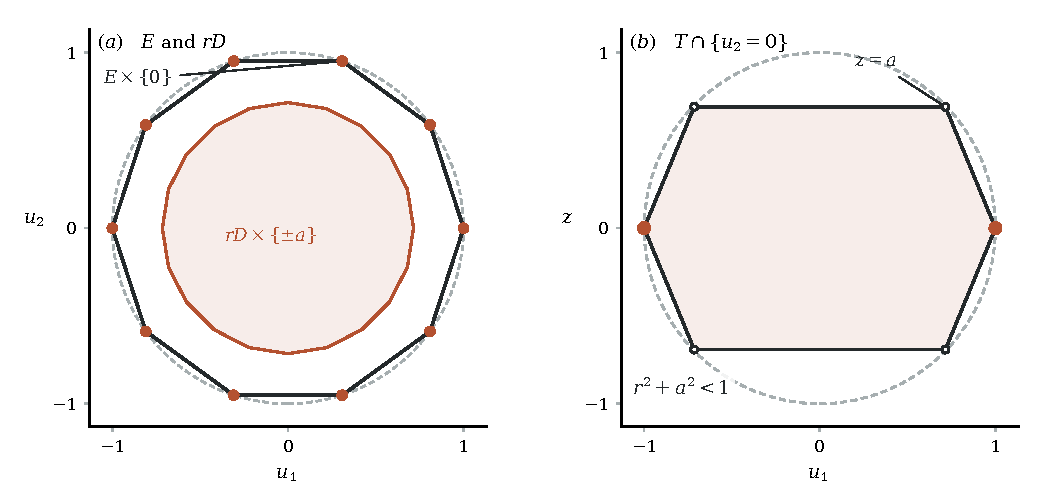
\includegraphics[width=.96\linewidth]{figures/affine-outer-body.pdf}
 \caption{The outer projection body $T$: its middle and end polygons in
 plan view, and an axial section inside the unit-ball section. Only the
 ten equatorial vertices meet the sphere.}
 \label{fig:affine-outer}
\end{figure}


\begin{proposition}[Projection certificate]
\label{prop:affine-projection}
The full action polar satisfies
\[
 U(\mathcal C)\subset T\subset\overline B^3(1).
\]
Moreover $T\cap S^2$ consists of exactly the ten vertices of
$E\times\{0\}$.
\end{proposition}

\begin{proof}
First describe $T$ without computation. Since $rD\subset E$, its slice at
height $|z|=a\tau$, for $0\leq\tau\leq1$, is
$(1-\tau)E+\tau rD$. One way to verify this slice identity is to replace
a mixture of the upper and lower copies of $rD$ by a point of $E$ at
height zero; the remaining mixture has the stated form.
The edge normals of the planar Minkowski sum are the union of the edge
normals of its two summands. Thus a complete halfspace description of $T$
is $|z|\leq a$, together with
\begin{equation}
 n\cdot u+\frac{d_0-d_1}{a}|z|\leq d_0,
 \qquad d_0=h_E(n),\quad d_1=rh_D(n),
 \label{eq:affine-outer-halfspaces}
\end{equation}
for every edge-normal direction of $E$ or $D$. There are $62$ halfspaces:
two horizontal ones and two for each of $30$ planar directions.
For exact coordinates, the edge normals of $E$ can be taken to be the odd
vertices of $D$, and those of $D$ to be sums of adjacent vertices of $D$.

The vertices in the middle level of $T$ have norm one, whereas all the
vertices in its upper and lower levels satisfy
\[
 |(ru,\pm a)|^2=r^2+a^2<1.
\]
Convexity proves $T\subset\overline B^3(1)$. Strict convexity of the ball
shows that its unit-sphere contacts are exactly the ten middle vertices.

It remains to place $U(\mathcal C)$ in these halfspaces. The finite
certificate described below supplies $18$ feasible action bivectors
$q_0b_j\in\mathcal W$. Write $Lx=U(x)$. For four representative
halfspaces $h_0+h\cdot y\geq0$, with $h_0>0$, it gives coefficients
$\lambda_j\geq0$ satisfying
\begin{equation}
 \sum_j\lambda_j=1,\qquad
 \sum_j\lambda_jb_j=-\frac{h^{\mathsf T}L}{h_0}.
 \label{eq:affine-dual-certificate}
\end{equation}
Every $x\in\mathcal C$ satisfies $b_j\cdot x\leq1$. Hence
\eqref{eq:affine-dual-certificate} implies the representative halfspace
inequality at $U(x)$.

The remaining halfspaces follow by symmetry. The projection
$U(\mathcal C)$ is invariant under the group generated by
\[
 (u,z)\longmapsto(R(2\pi/5)u,z),\qquad
 (u_1,u_2,z)\longmapsto(u_1,-u_2,z),\qquad
 y\longmapsto-y.
\]
Indeed, the first map is induced by congruence of $\Omega$ with the
$-2\pi/5$ rotation of the $q$ pentagon. The second is induced by the
negative of congruence with
$\operatorname{diag}(1,-1,-1,1)$, the simultaneous horizontal reflection
of the $q$ pentagon and vertical reflection of its partner. The last is
$\Omega\mapsto-\Omega$. The two congruences permute the facet normals
of $H$, and therefore permute the feasible words defining $\mathcal W$;
negation preserves its support function by word reversal. Substitution
in~\eqref{eq:affine-U} gives the claimed maps on $U$.
The four representatives have orbits of sizes $2,20,20,20$, covering all
$62$ halfspaces. The exact verification also checks these normal
permutations, projection identities, and orbit coverage.

The symmetry argument applies to the \emph{full} action polar
$\mathcal C$. The polyhedron defined only by the selected $18$ witness
inequalities need not be invariant under this group. No such invariance
is used. This proves $U(\mathcal C)\subset T$.
\end{proof}

\subsection{The finite predicate and its reproduction}
\label{subsec:affine-certificate}

All finite data lie in the ordered field
$F=\mathbb Q(t)$, where $t^4-10t^2+5=0$ and $0<t<1$. To specify the
geometry used by the certificate, put
\[
 \alpha=\frac{3-s}{2},\qquad \beta=\frac{t(1+s)}2,
 \qquad \delta=s-1.
\]
Define the five planar normals
\[
 u_0=(1,t),\quad u_1=(-\alpha,\beta),\quad u_2=(-\delta,0),\quad
 u_3=(-\alpha,-\beta),\quad u_4=(1,-t).
\]
The ten four-dimensional normals are
$a_i=(u_i,0)$ and $a_{5+i}=(0,R(-\pi/2)u_i)$ for $0\leq i<5$.
For each of the $18$ witnesses the verifier checks distinctness of the
facet indices, nonnegativity and normalization of the weights, closure,
and the exact bivector identity~\eqref{eq:affine-action-witness}.
It then checks the four positive relations
\eqref{eq:affine-dual-certificate}. The words and field coefficients are
stored in \path{certificates/affine-hko/certificate.json}; they are finite proof
inputs rather than requests to run an optimizer.

For a compact description of the four relations, let
$C=\cos(\pi/10)$, $S=\sin(\pi/10)$ and $\eta=S/(1+C)$.
Table~\ref{tab:affine-four-relations} gives the representative inequalities,
their support sizes, and simple exact lower bounds on every nonzero weight.
The first relation averages the two pure-factor five-facet witnesses with
weights $1/2,1/2$. The remaining coefficients are longer elements of $F$;
their complete values are retained in the certificate.

\begin{table}[ht]
\centering
\small
\begin{tabular}{@{}lrrr@{}}
\toprule
Representative halfspace in $(u_1,u_2,z)$
 & Witnesses & Weight lower bound & Orbit size\\
\midrule
$a+z\geq0$ & 2 & $1/2$ & 2\\
$C-u_2+(C-r)z/a\geq0$ & 4 & $1/40$ & 20\\
$1-u_1-\eta u_2+(1-r)z/a\geq0$ & 6 & $1/200$ & 20\\
$1-u_1-\eta u_2-(1-r)z/a\geq0$ & 6 & $1/30$ & 20\\
\bottomrule
\end{tabular}
\caption{Four exact convex combinations imply the complete outer-body
containment by symmetry. The bounds in the third column are not substitutes
for the exact identities.}
\label{tab:affine-four-relations}
\end{table}

The standalone SageMath program verifies the finite data from one JSON
input file. It reconstructs the facet normals,
all witness bivectors, the outer vertices and halfspaces, and the symmetry
actions. It accepts exactly the predicates used above: $18$ feasible
witnesses, four positive relations, coverage of $62$ halfspaces, and the
sphere bounds for $50$ outer vertices with precisely ten unit contacts.
It requires neither numerical optimization nor an external polyhedral
hull computation. Run \path{certificates/affine-hko/verify.py} with a
Python interpreter providing \texttt{sage.all}; it reads the sibling JSON
and records an execution summary. A successful run validates the
finite predicates; the slice argument, symmetry implication, and affine
capacity reduction are the mathematical steps proved in this section.

\subsection{Proof of the sharp bound and equality}

\begin{proof}[Proof of Theorem~\ref{thm:affine-hko}]
First suppose $\det A>0$ and let
$x=A^{-1}JA^{-\mathsf T}$ in skew-form coordinates. Put
$q=h_{\mathcal W}(x)/q_0>0$. By definition $x/q\in\mathcal C$, so
Proposition~\ref{prop:affine-projection} and
\eqref{eq:affine-split-norm} give
\[
 \mathfrak p(x)=|U(x)|^2-|V(x)|^2\leq |U(x)|^2\leq q^2.
\]
Equations~\eqref{eq:affine-ratio-formula} and
\eqref{eq:affine-hko-normalization} prove the claimed upper bound.

If equality holds, both inequalities are equalities. Thus $V(x)=0$, and
$U(x)/q$ is one of the ten unit-sphere contacts of $T$. Consequently
$x/q$ has zero same-factor entries and cross block
\begin{equation}
 \begin{pmatrix}
 \cos(k\pi/5)&\sin(k\pi/5)\\
 -\sin(k\pi/5)&\cos(k\pi/5)
 \end{pmatrix},\qquad k=0,\ldots,9.
 \label{eq:affine-equality-forms}
\end{equation}
Each is $T_0^{-1}JT_0^{-\mathsf T}$ for a linear automorphism $T_0$ of
$H$. Rotations by $2\pi/5$ in one factor give five of the forms; the
simultaneous factor reflections used above preserve $H$ and send $J$ to
$-J$, giving the other five. Therefore
\[
 A^{-1}JA^{-\mathsf T}=qT_0^{-1}JT_0^{-\mathsf T}.
\]
The matrix $S_0=\sqrt q\,AT_0^{-1}$ satisfies $S_0JS_0^{\mathsf T}=J$
and is symplectic. Hence $AH=q^{-1/2}S_0H$.
Conversely, symplectic images and positive dilations preserve $\rho$.

Finally, if $\det A<0$, compose $A$ on the right with
$\operatorname{diag}(1,-1,1,1)$. This is a determinant
$-1$ automorphism of $H$, so it changes the determinant sign without
changing $AH$. The positive-determinant argument applies. Translation
invariance gives the last assertion.
\end{proof}

% Frozen contribution: geometry_frontiers, 29 October 2026.
% Integrate after affine-hko-section.tex. Uses that section's action-body lemma.
% Certificate: exact_triangles_compact.py (Sage QQ/PPL).
\section{A product whose optimal affine position is not Lagrangian}
\label{sec:nonlagrangian-product}

The affine optimality of the pentagon product does not follow from a general
principle reducing products to Lagrangian position. Even a product of two
triangles has an affine image whose systolic ratio exceeds that of every
Lagrangian position of the same product. Here ``Lagrangian position'' means
that both original factor planes become Lagrangian; all independent affine
changes within those planes are allowed.

\begin{theorem}\label{thm:nonlagrangian-triangles}
Let
\[
 \Delta=\{(s,t)\in\mathbb R^2:s\leq1,\ t\leq1,\ -s-t\leq1\},
 \qquad K=\Delta\times\Delta.
\]
Among invertible linear maps $B$ for which both factor planes of $BK$
are Lagrangian, the maximum systolic ratio is $2/3$. The matrix
\[
 A=\begin{pmatrix}
 1&0&0&0\\
 1&-1&1&0\\
 0&1&0&0\\
 -1/4&-1/2&0&-1/4
 \end{pmatrix}
\]
satisfies
\[
 c_{\EHZ}(AK)=\frac{27}{10},\qquad
 \Vol_4(AK)=\frac{81}{16},\qquad
 \rho(AK)=\frac{18}{25}>\frac23.
\]
Consequently, no maximum of the systolic ratio on the full affine orbit
of $K$ occurs in Lagrangian position. By affine equivalence, the same
conclusion holds for the product of any two nondegenerate triangles.
\end{theorem}

The comparison covers \emph{every} Lagrangian position. Both ratios are below
one, so the result gives no Viterbo counterexample. It does not compute the
full affine maximum.

\subsection{Closure and the explicit non-Lagrangian image}

Use the conventions of Lemma~\ref{lem:affine-action-body}. The area of
$\Delta$ is $9/2$, so $\Vol_4(K)=81/4$. Its six support-normalized normals are
\[
 a_0=e_1,\quad a_1=e_2,\quad a_2=-e_1-e_2,\qquad
 a_3=e_3,\quad a_4=e_4,\quad a_5=-e_3-e_4.
\]
Closure forces every feasible weight vector to have the form
\begin{equation}\label{eq:triangle-product-weights}
 \beta_0=\beta_1=\beta_2=\frac t3,\qquad
 \beta_3=\beta_4=\beta_5=\frac{1-t}{3},\qquad 0\leq t\leq1.
\end{equation}
Cyclic shifts of an order do not change its action: the change caused by
moving its first weighted normal to the end is its pairing with twice the
sum of the remaining weighted normals, which vanishes by closure. Thus the
$120$ orders starting with $0$ cover all orders. The endpoints in
\eqref{eq:triangle-product-weights} include smaller supports.

For $x=(1,1,-2,1,1,-1)$, direct multiplication gives
\[
 \Omega=A^{-1}JA^{-\mathsf T},\qquad
 \det A=\frac14,\qquad \mathfrak p(x)=4.
\]
For each order its action is
\[
 Q_\sigma(t)=\frac19\bigl[a t^2+b(1-t)^2+d t(1-t)\bigr],
 \qquad a,b\in\{-1,1\}.
\]
The following finite table gives the greatest mixed coefficient $d$ in
each of the four groups. Each group contains $30$ cyclic orders. A witness
in every row also makes the bound sharp in that group.
\begin{center}
\begin{tabular}{ccclc}
\toprule
$a$&$b$&$\max d$&Attaining order&$\max_{\sigma,t} Q_\sigma(t)$\\
\midrule
$1$&$1$&$4$&$(0,1,3,2,5,4)$&$1/6$\\
$1$&$-1$&$6$&$(0,5,1,3,2,4)$&$5/27$\\
$-1$&$1$&$6$&$(0,3,2,5,1,4)$&$5/27$\\
$-1$&$-1$&$4$&$(0,2,5,1,3,4)$&$1/18$\\
\bottomrule
\end{tabular}
\end{center}
All entries follow by summing the $15$ pairings of the listed six normals;
the accompanying exact verifier enumerates precisely these $120$ orders.
Since $t(1-t)\geq0$, the maximum mixed coefficient bounds the whole group.
The four elementary quadratic maxima occur at $t=1/2,2/3,1/3,1/2$,
respectively. Therefore the full Haim--Kislev maximum is
\[
 h_{\mathcal W_K}(x)=\frac5{27}.
\]
The affine capacity formula gives $c_{\EHZ}(AK)=27/10$, and the volume and
ratio in the theorem follow. The table proves the required global capacity
calculation, rather than merely exhibiting one feasible action.

\subsection{The entire Lagrangian subclass}

For a nondegenerate skew matrix, both diagonal $2\times2$ blocks vanish
if and only if both diagonal blocks of its inverse vanish. Since
$B^{\mathsf T}JB=-\Omega^{-1}$, the two factor planes are Lagrangian exactly
when
\[
 \Omega=\begin{pmatrix}0&M\\-M^{\mathsf T}&0\end{pmatrix},\qquad
 M\in GL(2,\mathbb R).
\]
Conversely, every such $M$ occurs, by taking $B=\operatorname{diag}(M^{-1},I_2)$.
Write $h(M)$ for the action support at this cross form. Homogeneity and
$|\det B|^{-1}=|\det M|$ give
\begin{equation}\label{eq:triangles-cross-ratio}
 \rho(BK)=\frac{|\det M|}{162h(M)^2}.
\end{equation}

The same-factor terms now vanish, so each order has action
$t(1-t)$ times a linear form in $M$. Reversal of an order negates this
linear form. Consequently the global maximum occurs at $t=1/2$, and
$h(M)$ is a finite support function. Set
\[
 C=\{M:h(M)\leq1/12\},\qquad
 u_1=(1,0)^{\mathsf T},\quad u_2=(0,1)^{\mathsf T},\quad
 u_3=(1,-1)^{\mathsf T}.
\]
The second finite identity used in the proof is
\begin{equation}\label{eq:triangles-rankone-hull}
 C=\conv\left\{\pm\frac32u_i u_j^{\mathsf T}:1\leq i,j\leq3\right\}.
\end{equation}
To verify it exactly, form the $120$ action rows at weights $1/6$, multiply
them by $12$, and impose their upper bounds $1$. Rational polyhedral
reduction gives a bounded four-dimensional polytope with $30$ facets and
exactly the $18$ vertices displayed in \eqref{eq:triangles-rankone-hull}.
The verifier asserts equality of these two vertex sets, not an approximate
match. This finite hull identity is the only polyhedral calculation used
in the following determinant bound.

Let $D=\conv\{\pm u_1,\pm u_2,\pm u_3\}$. Grouping any convex combination
in \eqref{eq:triangles-rankone-hull} by its first index writes
\[
 M=\frac32\sum_{i=1}^3u_i v_i^{\mathsf T},\qquad
 v_i\in\alpha_i D,\quad \alpha_i\geq0,\quad\sum_i\alpha_i=1.
\]
Each determinant of two vertices of $D$ has absolute value at most one.
By bilinearity and convexity this implies $|\det(v_i,v_j)|\leq\alpha_i\alpha_j$.
The two-dimensional Cauchy--Binet identity now yields
\[
 |\det M|
 \leq\frac94\sum_{i<j}|\det(u_i,u_j)|\,|\det(v_i,v_j)|
 \leq\frac94\sum_{i<j}\alpha_i\alpha_j
 \leq\frac34.
\]
The last step follows from $\sum_i\alpha_i^2\geq1/3$.
Equality is attained by $\alpha_i=1/3$ and $v_i=u_i/3$, giving
\[
 M_* =\frac12\sum_i u_i u_i^{\mathsf T}
 =\begin{pmatrix}1&-1/2\\-1/2&1\end{pmatrix},\qquad
 \det M_*=\frac34.
\]
It also has $h(M_*)=1/12$: a smaller value would allow dilation within $C$
and contradict the determinant bound. For any nonzero $M$, the matrix
$M/(12h(M))$ belongs to $C$. Equation~\eqref{eq:triangles-cross-ratio} therefore
gives
\[
 \rho(BK)\leq\frac{144}{162}\cdot\frac34=\frac23,
\]
with equality for $M_*$. This proves the sharp global comparison.

Finally, a full affine maximum exists. By
Lemma~\ref{lem:affine-action-body}, the action support is a norm. The continuous
function $|\Pf|$ attains a positive maximum on its compact unit ball. Any
maximizing form is nondegenerate and hence is congruent to the standard
symplectic form; it is realized by an invertible linear image. Since its
ratio is at least $18/25$, no maximizing position has Lagrangian factor planes.

\paragraph{Exact checks and scope.}
The retained verifier
\path{certificates/triangle-position/exact_triangles_compact.py}
uses rational arithmetic
and Sage's PPL backend to reconstruct both finite identities from the six
normals. It verifies the four action-coefficient groups, the explicit matrix,
and the $18$-vertex identity. An independent calculation also checks the
global determinant maximum by enumerating stationary points on faces of
dimensions at most two. The proof above replaces that larger face calculation
by Cauchy--Binet. These checks do not establish priority in the literature.
Published bounds for triangle--convex Lagrangian products concern a different
comparison class. The bounded source comparison is recorded at
\path{reviews/triangle-position-prior-comparison.md}; it does not establish
priority.

% Frozen main-section module, 29 October 2026.
% Requires amsmath, amssymb, amsthm; theorem, lemma, proposition environments.
% General derivative appendix supplies Theorem thm:mc-derivative.
\section{A simultaneous-cut improvement of the pentagon product}
\label{sec:hko-ascent}

The explicit twenty-facet body $H_{3/10}$ in
Theorem~\ref{thm:hko-finite-improvement} has ratio
$1.051914\ldots>(3+\sqrt5)/5$, although the pentagon product maximizes
its entire affine orbit. The finite-parameter capacity computation is
separate from local behavior at the product. We prove that the product is
not a local maximum when the number of facets is unrestricted by studying
the right derivative of a fixed twenty-row family. The calculation combines
the simultaneous-splitting derivative with a reduction tailored to its cut
profiles and an exhaustive exact calculation of the remaining
shortest-word responses.

The complex structure $\mathbb{J}$ below is the one in the appendix,
whose matrix is the negative of the skew-form matrix $J$ in
Section~\ref{subsec:affine-action-body}.

Let $P\subset\mathbb R^2$ be the regular pentagon with vertices
$(\cos(2\pi k/5),\sin(2\pi k/5))$, $0\leq k<5$, and let
$J_2(x,y)=(-y,x)$. In coordinates $(q,p)$ put
\[
 H=P\times_L(-J_2P),\qquad
 \mathbb{J}(q,p)=(-p,q),\qquad \tau=\tan(\pi/5).
\]
Let $n_i$ be the support-normalized outward normal of the edge from vertex
$i$ to vertex $i+1$ of $P$, with indices taken modulo five, and set
$m_i=-J_2n_i$. Thus $n_0=(1,\tau)$ and
$|n_i|=|m_i|=\sqrt5-1$. The ten normals of $H$ are
$a_i=(n_i,0)$ and $a_{5+i}=(0,m_i)$. Define
\begin{align}
 D_i&=\left(-\frac35n_i,\frac{J_2n_i}{|n_i|}\right),&
 D_{5+i}&=\left(-\frac{J_2m_i}{|m_i|},-\frac35m_i\right),
 \label{eq:ha-directions}\\
 H_t&=\{x:a_j\cdot x\leq1,\ (a_j+tD_j)\cdot x\leq1,
                         \ 0\leq j<10\}.\label{eq:ha-family}
\end{align}
Every old inequality is retained, so $H_t\subset H$ for $t\geq0$.
For sufficiently small $t$ these are full-dimensional bounded polytopes and
$H_t\to H$ in Hausdorff distance. Equivalently,
\[
 H_t=H\cap L_t^{-1}H,\qquad
 L_t=\begin{pmatrix}aI_2&-bJ_2\\ bJ_2&aI_2\end{pmatrix},\quad
 a=1-\frac35t,\quad b=\cos(\pi/5)t.
\]
There are exactly twenty genuine facets for all sufficiently small $t>0$.
Indeed, on the relative interior of each old facet, $D_i\cdot x$ takes
both positive and negative values on open patches. A negative patch retains
the old facet with every competing inequality strict. At a positive patch,
the point $x/(1+tD_i\cdot x)$ lies on the new hyperplane, strictly satisfies
the old inequality, and keeps all other inequalities strict for small $t$.
Thus each old and each new row supports a facet.
Write $\operatorname{sys}(K)=c_{\mathrm{EHZ}}(K)^2/
(2\operatorname{Vol}_4(K))$.

\begin{theorem}[Strict inward ascent]\label{thm:ha-ascent}
For the family~\eqref{eq:ha-family},
\begin{equation}\label{eq:ha-slope}
 \left.\frac{d}{dt}\right|_{0+}\log\operatorname{sys}(H_t)
       =\frac{20+64\sqrt5}{9375}>0.
\end{equation}
Consequently $\operatorname{sys}(H_t)>\operatorname{sys}(H)$ for every
sufficiently small positive $t$. In particular, $H$ is not a local maximum
among convex bodies in the Hausdorff topology.
\end{theorem}

The statement concerns twenty facets and does not contradict the
separately proved local maximum among convex four-polytopes with at most
eleven genuine facets.\footnote{Computer-assisted proof and independent
acceptance record:
\path{evidence/historical-comparisons/f11/README.md}.}
The existence of a small improving interval follows from the positive
derivative. Proposition~\ref{prop:hko-effective} in the quantitative appendix
also supplies an explicit near-zero subinterval for this family.

\subsection{The cut profile and the repeated-word issue}

On each original facet the inward profile is
\begin{equation}\label{eq:ha-profile}
 f_i=(\ell_i-3/5)_+,\qquad
 \ell_i(q,p)=\frac{J_2n_i}{|n_i|}\cdot p,
 \qquad
 f_{5+i}=(\ell_{5+i}-3/5)_+,\quad
 \ell_{5+i}(q,p)=-\frac{J_2m_i}{|m_i|}\cdot q.
\end{equation}
These profiles are convex on their respective facets and constant along
their own characteristic directions $\mathbb{J}a_i$. The constancy is essential:
general convex profiles need not admit the reduction below.

Use the active-word action
$Q(\sigma,\beta)=\sum_{r<s}\beta_r\beta_s
\langle \mathbb{J}a_{\sigma_r},a_{\sigma_s}\rangle$, with
$\sum\beta_ra_{\sigma_r}=0$, $\sum\beta_r=1$, and $\beta_r\geq0$.
Write $Q_*=1/(2c_{\mathrm{EHZ}}(H))=\tau/5$.
For a maximizing word, $\mu_\gamma$ denotes its normalized-time occupation
measure on the disjoint union of labeled facets. The general derivative
theorem uses all finite maximizing words, including repeated labels;
an existence theorem for a simple shortest word alone would not suffice.

\begin{lemma}[Removal of repeated visits]\label{lem:ha-repeat}
Let $K$ be a Lagrangian product of planar polygons with no antipodal facet
normals. Suppose each continuous convex facet profile is constant on lines
parallel to its own characteristic direction. Every finite maximizing word
has a simple maximizing word with at least as large an occupation response.
The same supremum therefore bounds the weak closure of the finite-word
occupation measures.
\end{lemma}

\begin{proof}
Delete zero weights. Suppose a full normal $a=(n,0)$ occurs twice, at
positions $r<s$. Transfer weight by
$\beta_r(z)=\beta_r+z$, $\beta_s(z)=\beta_s-z$ on
$[-\beta_r,\beta_s]$, fixing all other weights. Closure and normalization
are preserved. The action is affine in $z$, since its quadratic coefficient
pairs $a$ with itself. The repeated-word polar-loop bound $Q\leq Q_*$,
together with the interior maximum at $z=0$, makes this affine function
constant. Equality of the normals alone would not imply constancy.

At every interior parameter, the active normals span both factor planes:
a positive closed combination without antipodal directions contains at least
three distinct directions. The augmented normal matrix has rank five,
because averaging a relation $u\cdot a_j+c=0$ against the positive weights
first gives $c=0$, then $u=0$. Thus the KKT multiplier $\lambda(z)$ is unique
and affine in $z$. With $T=(2Q_*)^{-1}$, the reconstructed vertices are
\[
 x_k(z)=-T\lambda(z)+2T\mathbb{J}\sum_{j<k}\beta_j(z)a_{\sigma_j}.
\]
They lie in $K$ on their labeled facets by the reconstruction argument in
Theorem~\ref{thm:mc-derivative}.

Choose the cyclic start just before the first duplicate and put $v=2T\mathbb{J}a$.
Every fixed-weight segment translates with derivative $u$ or $u+v$,
according to which interval between the duplicates contains it. All
q-facet equations give $n_j\cdot u_q=0$, so $u_q=0$. The p-facet equations
give $m_j\cdot u_p=0$ outside the interval and
$m_j\cdot(u_p+v_p)=0$ inside. There are at least three distinct p-normal
directions; one interval contains two nonparallel ones. Hence $u_p=0$ or
$u_p=-v_p$, and therefore $u=0$ or $u=-v$.

Both duplicate segments consequently move and change length only along
their own characteristic direction. Their profile values $c_r,c_s$ stay
constant, and their combined response
$(\beta_r+z)c_r+(\beta_s-z)c_s$ is affine. Every other weight is fixed and
its segment translates affinely; integrating its convex profile gives a
convex function of $z$. The total response is convex. By continuity it
extends to the endpoints, where the zero-weight occurrence is deleted.
One endpoint has at least the original response. The p-normal case is
identical with the factors exchanged. Iteration removes all repetitions.
Continuity on the compact disjoint facet union passes the bound to weak
limits of the occupation measures.
\end{proof}

\subsection{Complete calculation of the simple-word response}

\begin{proposition}[Exact finite response certificate]\label{prop:ha-certificate}
For the profiles~\eqref{eq:ha-profile},
\begin{equation}\label{eq:ha-response}
 \max_{\text{simple maximizing }\gamma}\int f\,d\mu_\gamma=\frac1{125}.
\end{equation}
The complete maximizing weight family is covered by 190 charts: 50 points
on six-label words and 140 closed intervals on seven-label words.
\end{proposition}

\begin{proof}
We describe both the exhaustive reduction and the exact predicates checked
by the accompanying portable certificate.
The normalized closure polytope in either factor is
\[
 C_q=\{u\geq0:\sum u_i=1,\ \sum u_in_i=0\},\qquad
 C_p=\{v\geq0:\sum v_i=1,\ \sum v_im_i=0\}.
\]
Its vertices have support at most three by rank of the three affine
constraints. No support of size one or two closes. Solving all ten
three-element supports gives precisely five positive vertices in each
factor, with exact weights in $\mathbb Q(\tau)$.

For a fixed word, split its weights as $(tu,(1-t)v)$. Same-factor pairings
vanish, so $Q=t(1-t)B_\sigma(u,v)$ with $B_\sigma$ bilinear.
Every positive global maximizer has $t=1/2$. Decomposing $u,v$ into closure
vertices expresses its value as a convex combination of triangle-pair
actions. Each pair action is at most $Q_*$, so every pair with positive
product coefficient must attain $Q_*$. Conversely, mixtures supported on
a complete bipartite set of winning pairs attain $Q_*$.

There are $25\cdot5!=3000$ triangle-pair cyclic six-orders. Exact evaluation
checks that all have action at most $\tau/5$, with precisely 50 equality
words. Every simple support word extends by zero weights to a cyclic
ten-order. Fixing label zero first gives all $9!=362880$ such orders.
For each, form the $5\times5$ graph of its winning induced triangle pairs.
Every maximizing weight pair is covered by a maximal complete bipartite
subgraph. These are enumerated as follows: for every nonempty row subset
$R$, form its common-neighbor set $C$, retain it when $C\ne\varnothing$
and $R$ is exactly the common-neighbor set of $C$. This is precisely the
maximality condition. Delete labels absent from the union of its triangle
supports and deduplicate by the remaining cyclic word and the two vertex
subsets. This loses no maximizing weight or response.

The exhaustive scan gives 79494 orders with winning pairs, 121 distinct
nonempty pair graphs, and 190 distinct charts. Fifty charts use one closure
vertex in each factor. Seventy use two q-vertices and one p-vertex; seventy
use one q-vertex and two p-vertices. No other chart occurs. Thus every
nonconstant weight family is an interval $\beta(z)=b+zd$, $0\leq z\leq1$.
The catalogue argument needs only the convex hull of the two vertices,
not an additional assertion about adjacency in the closure pentagon.

On each chart, solve the rank-five KKT equations exactly. The multiplier
and orbit vertices are affine in $z$, as are the radial coordinates
$\ell_i(z)$. Each radial coordinate is constant along its labeled segment.
The response therefore has the form
\[
 R(z)=\sum_i(b_i+zd_i)\max(0,h_i+zk_i).
\]
Partition $[0,1]$ at every exact hinge zero. On each resulting interval
$R$ is quadratic. Its maximum is attained at an endpoint or at the interior
stationary point of a strictly concave quadratic. The checker evaluates all
these candidates with exact field arithmetic and isolated signs for the
root $0<\tau<1$ of $\tau^4-10\tau^2+5=0$.
Of the 190 chart maxima, 110 equal zero and 80 equal $1/125$.
For example, the chart with word $(0,6,5,2,1,8,4)$ attains $1/125$ at
the parameter $z=3/10-\tau^2/50$ in the certificate's endpoint ordering.
This proves~\eqref{eq:ha-response}.
\end{proof}

The portable replay at \path{certificates/hko-ascent/README.md}
contains the literal normal construction, all positive
triangle weights, the complete cyclic-order enumeration, and the exact
piecewise-quadratic calculation. It requires Python's standard library and
a C++17 compiler. Its checker recomputes all outputs in a fresh output
directory and compares them with the retained certificate. A separate
Sage-field and Python enumeration reproduced the complete 190-chart set;
an independent replay also reproduced all exact response maxima. These
checks support the stated finite predicates; the coverage implication is
the argument above.

\subsection{Volume and the strict derivative}

\begin{proof}[Proof of Theorem~\ref{thm:ha-ascent}]
Each labeled facet has normalized cone-volume mass $1/10$. Its profile is
independent of the edge coordinate and cuts a cap from the other pentagon.
The cap depth is $\delta=2/5<1-\cos(2\pi/5)$, so the cap is a triangle
with area $\delta^2\cot(\pi/5)$. The hinge's mean on this triangle is
$\delta/3$, and the pentagon area is $A=5\tau/(1+\tau^2)$. All ten facet
averages agree. Consequently
\begin{equation}\label{eq:ha-volume}
 \int f\,d\nu=\frac{\delta^3}{3\tau A}
             =\frac8{625}-\frac{8\tau^2}{9375}.
\end{equation}
Lemma~\ref{lem:ha-repeat} and Proposition~\ref{prop:ha-certificate} identify
the supremum over all finite maximizing words, and hence their weak closure,
with $1/125$. The full-rank support hypothesis of
Theorem~\ref{thm:mc-derivative} holds because both planar normal sets have no
antipodal pairs. That theorem applies directly to the fixed twenty-row bank:
\[
 D^+\log\operatorname{sys}(H_t)
 =4\left(\frac8{625}-\frac{8\tau^2}{9375}-\frac1{125}\right)
 =\frac{20+64\sqrt5}{9375}>0.
\]
Since $H_t\to H$, the definition of a positive right derivative gives the
claimed strict improvements arbitrarily close to $H$.
\end{proof}

% Owned contribution: geometry_frontiers. Insert after the HKO ascent section.
% Uses eq:ha-family and the article's standard macros. Citation: Lawrence1991.
\subsection{An explicit finite improvement}
\label{subsec:hko-finite-improvement}

The same fixed family also gives a visible improvement at a moderate
parameter; this does not follow from the positive derivative alone.
For $H_t$ in \eqref{eq:ha-family}, we certify the capacity at $t=3/10$.
The capacity decreases slightly, but the volume decreases by enough to raise
the systolic ratio.

\begin{theorem}[A twenty-facet improvement of HKO]
\label{thm:hko-finite-improvement}
Let $K=H_{3/10}$ and $\tau=\tan(\pi/5)$. Then $K$ is a simple convex
four-polytope with twenty facets and seventy-five vertices, and
\[
 c_{\EHZ}(K)=\frac{1019}{410\tau}
           =\frac{1019}{1025}c_{\EHZ}(H),\qquad
 \Vol_4(K)=\frac{502711205+99664289\sqrt5}{130445600}.
\]
Its systolic ratio satisfies
\[
 \rho(K)=1.0519141388294875\ldots
        >\rho(H)=\frac{3+\sqrt5}{5}.
\]
More precisely,
\[
 \rho(K)-\rho(H)
 =\frac{7965280+4064064\sqrt5}
        {5(502711205+99664289\sqrt5)}>0.
\]
\end{theorem}

This is a complete capacity computation for one body, rather than an
upper bound obtained from one closed characteristic. It does not optimize
$t$ or assert a sharp upper bound for all convex bodies.

\begin{proof}
Write the twenty support-normalized normals as
\[
 N=(a_0,\ldots,a_9,a_0+\tfrac3{10}D_0,\ldots,
                    a_9+\tfrac3{10}D_9).
\]
Denote the row with label $i\in\{0,\ldots,19\}$ by $n_i$.
The exact calculation uses the number field
$\mathbb Q(\tau)$ with $\tau^4-10\tau^2+5=0$ and $0<\tau<1$.
We describe both the finite predicates and the argument that makes them
complete.

\emph{Geometry.}
Solving every invertible four-row subsystem of $Nx\leq\mathbf1$ and testing
all twenty inequalities gives seventy-five vertices. Exactly four linearly
independent rows are active at every vertex, and all twenty labels occur.
This proves simplicity and that every listed inequality defines a genuine
facet. It also determines all nonempty pairwise facet intersections.

\emph{Which words need checking.}
Haim--Kislev's geometric simple-minimizer theorem~\cite[Theorem~1.5]{HK2017} provides a minimizing
characteristic using each facet velocity at most once. Consecutive facet
labels $i,j$ must meet and satisfy $\omega(n_i,n_j)\geq0$: the arriving
segment reaches the $j$th support hyperplane from inside the body.
The exact transition graph has $120$ directed edges, including zero-pairing
edges. Thus some capacity-maximizing word is a simple cycle of this graph.

For a word, let $C\beta=e$ be closure and normalization, and let
$Q(\beta)=\tfrac12\beta^{\mathsf T}G\beta$. If
$z\in\ker C$ has $z^{\mathsf T}Gz>0$, the word cannot have an interior
maximum. Zero extension of $z$ gives the same obstruction for every
larger word containing it in cyclic order. The certificate verifies
$77\,927$ symmetry representatives of such obstructions by exact nullspace
and quadratic-form calculations. Cyclic invariance on the constraint
kernel follows from closure; the twenty symmetry actions are checked exactly.

An integer depth-first traversal then enumerates all simple cycles, stopping
only at a certified obstructed prefix. Every remaining cycle occurs in the
checked list. The traversal covers $43\,110$ cycles, represented by $2326$
words after symmetry, with no unaccounted cycle. This coverage check uses no
floating-point curvature decision.

\emph{The scalar maximum on each remaining word.}
Deleting zero weights from the geometric maximizing word places it in the
relative interior of its searched active cycle. Thus boundary maxima are
covered by their positive support.
After removing dependent equality constraints, every interior maximum obeys
\[
 G\beta+C^{\mathsf T}\lambda=0,\qquad C\beta=e.
\]
For an invertible KKT matrix the solution is computed exactly; a negative
weight excludes that stationary point. Singular systems are handled as
affine families. Their objective is constant: a kernel element $(z,\eta)$
satisfies $Cz=0$, $Gz+C^{\mathsf T}\eta=0$, and hence $e\cdot\eta=0$.
Consequently $Q=-e\cdot\lambda/2$ has the same value throughout the family.

Of the $1030$ singular families, $984$ have objective at most the target
$205\tau/1019$. Another $21$ are infeasible by the elementary inclusion
\[
 \frac{25}{28}H\subset K,
 \qquad Q_{\max}(K)\leq\frac\tau5\left(\frac{28}{25}\right)^2.
\]
Indeed, every moving normal has support at most
$1+(2/5)(3/10)=28/25$ on $H$.
The remaining $25$ families are proved infeasible by exact vertex enumeration
in their free parameters. This is exhaustive: their nonnegative weights
would lie in the compact simplex, the parameter map is injective, and any
nonempty bounded parameter polyhedron has a vertex determined by independent
active zero-weight equations. Thus no singular or flat family is omitted.
The resulting global upper bound is
\[
 Q_{\max}(K)\leq\frac{205}{1019}\tau.
\]

Equality is witnessed by the word $(0,1,6,7,3,12,9)$ with positive weights
\[
 \frac1{8152}\bigl(
 1271+123\tau^2,\ 697+205\tau^2,\ 965+205\tau^2,\
 1070+190\tau^2,\ 1804-328\tau^2,\ 400,\
 1945-395\tau^2\bigr).
\]
The exact checks verify closure, normalization, positivity, and objective
$205\tau/1019$. The Haim--Kislev formula therefore gives the claimed capacity.

\emph{Volume and ratio.}
For a simple four-polytope, Lawrence's formula~\cite{Lawrence1991} is
\[
 \Vol_4(K)=\frac1{4!}\sum_v
 \frac{(\ell\cdot v)^4}
 {|\det N_{I(v)}|\prod_{j=1}^4(\ell N_{I(v)}^{-1})_j},
\]
where $I(v)$ lists the four active normals and $\ell$ is nonconstant on every
edge. Exact evaluations with $\ell=(1,2,4,8)$ and $(1,3,9,27)$ have nonzero
denominators and agree with the stated volume. Substituting the capacity
and simplifying in $\mathbb Q(\sqrt5)$ proves the displayed positive ratio
difference.
\end{proof}

The portable certificate at \path{certificates/hko-t03/README.md}
reconstructs the twenty normals, validates the
integer transition graph, checks every curvature exclusion and stationary
family, verifies the positive attaining weights, and recomputes the volume.
The coverage proof is independent of the numerical search that proposed the
word list. The computation concerns the exact algebraic body $H_{3/10}$;
it does not replace it by rounded input data.

% Frozen refinement module; requires hko-ascent-main.tex notation and results.
\subsection{Seventeen facets and the exact response to unequal cut speeds}
\label{subsec:hko-seventeen}

The twenty-row family admits a sharper facet-count conclusion. Keep the ten
profiles of~\eqref{eq:ha-profile} fixed, but give their new rows nonnegative
speeds $w=(w_0,\ldots,w_9)$:
\[
 H_{t,w}=\{x:a_i\cdot x\leq1,\
                 (a_i+tw_iD_i)\cdot x\leq1,\ 0\leq i<10\}.
\]
Its profile on facet $i$ is $w_if_i$. Write
\[
 \kappa=\int_{F_i}f_i\,d\nu
        =\frac{8(5+\sqrt5)}{46875};
\]
this value is independent of the facet and includes its cone-volume mass
$1/10$.

\begin{proposition}[Exact weighted response]\label{prop:ha-weighted}
For every $w_i\geq0$, the supremum over all finite maximizing words and their
weak occupation limits is
\begin{equation}\label{eq:ha-weighted-response}
 \sup_\gamma\sum_{i=0}^9w_i\int_{F_i}f_i\,d\mu_\gamma
       =\frac{\max_iw_i}{125}.
\end{equation}
Consequently
\begin{equation}\label{eq:ha-weighted-derivative}
 D^+\log\operatorname{sys}(H_{t,w})
       =4\left(\kappa\sum_iw_i-\frac{\max_iw_i}{125}\right).
\end{equation}
\end{proposition}

\begin{proof}
Nonnegativity and Proposition~\ref{prop:ha-certificate}, together with
Lemma~\ref{lem:ha-repeat}, give the upper bound
\[
 \sum_iw_i\int_{F_i}f_i\,d\mu_\gamma
 \leq(\max_iw_i)\int f\,d\mu_\gamma
 \leq\frac{\max_iw_i}{125}.
\]
For the reverse bound we exhibit a maximizing word whose entire response
is concentrated on one facet. Put $u=\tau^2$ and take
\begin{align*}
 \sigma&=(0,6,5,2,1,8,4),\\
 \beta&=\frac1{200}
 (17+5u,\ 25+5u,\ 25+5u,\ 44-8u,\ 8,\ 50-10u,\ 31+3u).
\end{align*}
The weights are strictly positive, sum to one, close the normal word, and
give $Q=\tau/5$. Its KKT reconstruction has constant radial hinge arguments,
in this order,
\[
 \ell_{\sigma_r}-\frac35
 =\frac1{40}(-59+5u,\ -9-5u,\ -9-5u,\ -9-5u,\
                       8,\ -9-5u,\ -45+3u).
\]
Since $0<u<1$, only the facet labeled $1$ contributes. Its weight is
$1/25$ and its hinge value is $1/5$, giving response $1/125$ on that facet
and zero on all others. These are literal exact predicates checked by the
supplementary witness replay; the same point is chart~11 of the complete
catalogue, at parameter $3/10-\tau^2/50$.

Simultaneous rotation of the q- and p-planes by $2\pi/5$ preserves $H$,
the symplectic form, and this labeled profile family. The symplectic
involution
\[
 S(q,p)=(J_2p,-J_2q)
\]
also preserves $H$ and exchanges facet $i$ with facet $5+i$, including
their cut velocities. These symmetries act transitively on the ten facets.
Thus every facet admits a shortest word with response $1/125$ concentrated
there. Choose a facet with maximal $w_i$ to obtain the lower bound in
\eqref{eq:ha-weighted-response}. The derivative formula follows from
Theorem~\ref{thm:mc-derivative} and the volume response
$\kappa\sum_iw_i$.
\end{proof}

\begin{corollary}[A seventeen-facet ascent]\label{cor:ha-seventeen}
Choose any seven of the ten cuts in~\eqref{eq:ha-directions}, with unit
speed, and omit the other three new rows. For all sufficiently small
positive $t$ the resulting body has seventeen genuine facets, and
\[
 D^+\log\operatorname{sys}(H_{t,w})
 =\frac{4(56\sqrt5-95)}{46875}>0.
\]
Within the cone of nonnegative speeds on these fixed ten profiles, seven
new rows is the smallest number that can give a positive first variation.
\end{corollary}

\begin{proof}
The exact comparisons are
\[
 6\kappa=\frac{240+48\sqrt5}{46875}
   <\frac{375}{46875}=\frac1{125}
   <\frac{280+56\sqrt5}{46875}=7\kappa.
\]
Seven unit speeds therefore give the displayed positive derivative. Every
selected new row and every old row is a genuine facet by the open-patch
argument following~\eqref{eq:ha-family}, so the facet count is seventeen.
If instead at most six speeds are nonzero and $w\ne0$, then
$\sum_iw_i\leq6\max_iw_i$, making
\eqref{eq:ha-weighted-derivative} strictly negative. This proves the claimed
minimal count for this fixed profile cone; it does not exclude ascent using
different profiles or a different perturbation with fewer new facets.
\end{proof}

\subsection{Two characteristic-invariant cuts}
\label{subsec:ha-two-hinge}

The seven-cut threshold above concerns ten fixed radial profiles. A
different obstruction applies to any two affine hinges that are
constant along their own facet characteristic directions. Affine
offsets, dependence on the facet-edge coordinate, and unequal cut
speeds are allowed. For a nonnegative function $f$ on the disjoint
labeled facet union, put
\[
 R(f)=\sup_\gamma\int f\,d\mu_\gamma,
\]
where the supremum runs over all finite maximizing words, equivalently
their weak occupation limits.

\begin{proposition}[Two invariant hinges]\label{prop:ha-two-hinge}
On one HKO facet $F_i$, let $f_i(x)=(D\cdot x)_+$, with $f$ zero on the
other labeled facets and $D\cdot\mathbb{J}a_i=0$. Then
\begin{equation}\label{eq:ha-amplification}
 R(f)\geq2\nu(f).
\end{equation}
Consequently, retain all ten original inequalities of $H$ and add at
most two rows $(a_i+tD)\cdot x\leq1$ satisfying this characteristic
invariance. Their one-sided first logarithmic systolic variation at
$t=0$ is nonpositive, whether the rows concern the same facet or
different facets.
\end{proposition}

Appendix~\ref{sec:ha-two-hinge-proof} proves the one-hinge bound from
four literal shortest-characteristic families and a scalar hinge
inequality, then handles both placements of two cuts. This is a
first-order obstruction for invariant affine hinges. It does not prove
local maximality among twelve-facet bodies, decide zero-derivative
directions at higher order, or cover non-invariant hinges.


\paragraph{Quantitative near-zero control.}
A uniform quadratic remainder for the true global optimal action makes the
positive first variation effective. For the original family with all ten
unit cuts it certifies $\rho(H_t)/\rho(H)>1+t/200$ when
$0<t\leq10^{-30}$. The pivot-and-rounding proof in
Appendix~\ref{sec:hko-effective} illustrates a quantitative sensitivity
method; this bound is not asserted for the seventeen-facet subfamilies.

% Candidate research section, 28 October 2026.
% Requires amsmath, amssymb, amsthm; theorem/lemma/proposition definitions supplied by wrapper.
% Independent component review in pfaffian/simplex-equality-audit.md.
\section{The simplex bound through a triangle-free graph}
\label{sec:simplex-sharp}

Haim--Kislev proved the sharp bound $c_{\mathrm{EHZ}}(K)^2/(2\operatorname{vol}_4K)
\leq3/4$ for every four-dimensional simplex in her 2019 MSc thesis
\cite[Theorem~B and Section~4]{HaimKislev2019CubesSimplices}. Her proof
uses pairing coordinates and a substantial sign-case analysis. Later
computations of Chaidez--Hutchings~\cite[Section~1.5]{CH2021} give
equality examples, while Leipold~\cite[Section~12.4]{Leipold2026}
reports numerical simplex values.
We give a different proof: the polar of the four-item linear-ordering
polytope has a triangle-free Pfaffian interaction graph. The graph bound
also yields the complete equality family below. The contribution here is
the proof mechanism and equality description, rather than the numerical
constant or its universal validity.

\begin{theorem}\label{thm:simplex-three-quarters}
Every nondegenerate simplex $K\subset\mathbb R^4$ satisfies
\[
 \frac{c_{\mathrm{EHZ}}(K)^2}{2\operatorname{vol}_4K}\le\frac34.
\]
The constant is sharp. In interleaved symplectic coordinates
$\omega_0=dz_1\wedge dz_2+dz_3\wedge dz_4$, equality holds precisely for
the images under translations, positive dilations and linear
symplectomorphisms of
\[
 K_{\mu,\nu}=\operatorname{conv}\{0,
 (1,0,\nu,-\nu),\ (0,1,-\mu,\mu),\ e_3,\ e_4\},
 \qquad \mu,\nu\ge0,\quad\mu+\nu\le1.
\]
\end{theorem}

\subsection{Barycentric gradients remove the weight optimization}

Let $\lambda_0,\ldots,\lambda_4$ be the barycentric coordinate functions of
$K$, and write $x_i=-d\lambda_i$ for their constant negative gradients,
identified with vectors using the ambient Euclidean coordinates. They obey
$\sum_{i=0}^4x_i=0$, and any four form a basis. Translate $K$ so that the
origin is interior, and set $\beta_i=\lambda_i(0)>0$. Its normalized facet
presentation is
\[
 K=\{z: a_i\cdot z\le1,\ 0\le i\le4\},
 \qquad a_i=x_i/\beta_i.
\]
The unique normalized nonnegative closure vector in Haim--Kislev's formula
is $(\beta_i)$: the kernel of the matrix of the five facet rows is
one-dimensional, and $\sum_i\beta_i=1$, $\sum_i\beta_i a_i=0$.

Define the alternating matrix
\[
 \Omega_{ij}=\omega_0(x_i,x_j),\qquad 1\le i,j\le4,
\]
and the order functional
\begin{equation}\label{eq:simplex-order-functional}
 S(\Omega)=\max_{\sigma\in\mathfrak S_4}
              \sum_{i<j}\Omega_{\sigma(i),\sigma(j)}.
\end{equation}
Closure makes cyclic rotation preserve the ordered pairing sum. Put $x_0$
last; its contribution is
$\omega_0(\sum_{i=1}^4x_i,x_0)=\omega_0(-x_0,x_0)=0$.
The Haim--Kislev formula~\cite[Theorem~1.1]{HK2017} therefore gives
\begin{equation}\label{eq:simplex-capacity-and-volume}
 c_{\mathrm{EHZ}}(K)=\frac1{2S(\Omega)},\qquad
 \operatorname{vol}_4K=\frac1{24|\operatorname{Pf}\Omega|}.
\end{equation}
For the second identity, the affine map
$z\mapsto(\lambda_1(z),\ldots,\lambda_4(z))$ takes $K$ onto the standard
simplex of volume $1/24$. Its absolute Jacobian is the absolute determinant
of the four gradients. The Pfaffian congruence identity gives the same
absolute determinant for $\Omega$. Thus
\begin{equation}\label{eq:simplex-ratio-pfaffian}
 \frac{c_{\mathrm{EHZ}}(K)^2}{2\operatorname{vol}_4K}
 =\frac{3|\operatorname{Pf}\Omega|}{S(\Omega)^2}.
\end{equation}
Conversely, every nondegenerate alternating matrix is a symplectic Gram
matrix of a basis, so this reduction describes the whole affine simplex
class. The gradients determine the labeled simplex up to translation;
equal Gram matrices identify them up to an affine symplectomorphism.

\subsection{The polar of the four-item ordering polytope}

Use coordinates $(12,13,14,23,24,34)$ on the six-dimensional space of
alternating matrices, and let $e_{ij}$ denote its coordinate unit vectors.
In these coordinates,
\[
 q(z):=\operatorname{Pf}z=z_{12}z_{34}-z_{13}z_{24}+z_{14}z_{23}.
\]
For $\sigma\in\mathfrak S_4$, let $p_\sigma$ have coordinate $+1$ on
$ij$ when $i$ precedes $j$ and $-1$ otherwise. Then $S$ is the support
function of $P=\operatorname{conv}\{p_\sigma\}$.

We use the classical facet description of the four-item linear-ordering
polytope: in incidence coordinates $y=(1+p)/2$, it is defined by
\[
 0\le y_{ij}\le1,\qquad
 0\le y_{ij}-y_{ik}+y_{jk}\le1\quad(i<j<k).
\]
After centering and polarity this says
\begin{equation}\label{eq:simplex-order-polar}
 C:=\{z:S(z)\le1\}=\operatorname{conv}\mathcal V,
 \quad
 \mathcal V=\{\pm e_{ij}:i<j\}\cup
 \{\pm(e_{ij}-e_{ik}+e_{jk}):i<j<k\}.
\end{equation}
There are twenty vertices. This small classical polytope identity is the
only ordering-polytope input needed below.
% Classical source: Groetschel--Juenger--Reinelt; Marti--Reinelt Ch.6.
% Independent exact rational active-basis certificate supplied separately.

For completeness, the facet description has a short integrality proof.
Let $R$ be the polyhedron defined by the displayed bounds and triangle
inequalities. At any vertex of $R$, some coordinate bound is active:
otherwise at most one constraint from each of the four triangle pairs can
be active, fewer than the six independent constraints needed at a vertex.
Relabeling the four items, we may suppose $y_{12}=1$. Write
$(a,b,c,d,e)=(y_{13},y_{14},y_{23},y_{24},y_{34})$.
On this face the remaining constraints are the unit box and
\[
 c\le a,\quad d\le b,\quad
 0\le a-b+e\le1,\quad 0\le c-d+e\le1.
\]
The four core row vectors are
\[
 \begin{pmatrix}
 1&0&-1&0&0\\
 0&1&0&-1&0\\
 1&-1&0&0&1\\
 0&0&1&-1&1
 \end{pmatrix}.
\]
Changing their signs by $(+,-,-,+)$ gives a matrix with one $+1$ and one
$-1$ in every column. Every square minor of such a directed-incidence
matrix is $0$ or $\pm1$: expand along a column with at most one nonzero
entry, or, if every column has two, use the zero sum of the rows.
Appending coordinate rows and signed copies preserves this property.
An invertible active constraint matrix consequently has determinant
$\pm1$, and its integer right-hand side forces the vertex coordinates
to be integers. Thus every vertex of $R$ is a zero--one vector. The
triangle inequalities exclude directed triangles; a tournament without
directed triangles is a total order. Hence $R$ is exactly the convex
hull of the twenty-four order vectors, proving
\eqref{eq:simplex-order-polar} without a computational assumption.

\subsection{A triangle-free Pfaffian interaction graph}

Let $f_1,\ldots,f_4$ be the standard basis of $\mathbb R^4$ and
$f_5=f_1+\cdots+f_4$. With the usual Hodge star,
\[
 \mathcal V=\{\pm*(f_i\wedge f_j):1\le i<j\le5\}.
\]
The six pairs not involving $f_5$ give the coordinate vectors; the other
four give the triangle vectors. Every vertex is decomposable and hence
has $q(v)=0$. Define its symmetric interaction with another vertex by
\[
 B(v,w)=q(v+w)-q(v)-q(w).
\]
If $v=\varepsilon*(f_i\wedge f_j)$ and
$w=\eta*(f_k\wedge f_l)$, then
\[
 B(v,w)=\varepsilon\eta\det(f_i,f_j,f_k,f_l).
\]
This is zero when the two index pairs intersect, and is $+1$ or $-1$
otherwise: every four distinct $f_i$ have determinant $\pm1$.

Let $G$ have vertex set $\mathcal V$, with $vw$ an edge exactly when
$B(v,w)=1$. It is triangle-free, since three pairwise disjoint two-element
subsets cannot fit inside a five-element set. It is also cubic: a pair has
three disjoint pairs, and exactly one sign of each gives positive
interaction. These elementary facts already prove the bound.

\begin{lemma}[Triangle-free weighted graph bound]\label{lem:simplex-graph-bound}
If $G$ is triangle-free and $\lambda_v\ge0$, $\sum_v\lambda_v=1$, then
\[
 \sum_{vw\in E(G)}\lambda_v\lambda_w\le\frac14.
\]
\end{lemma}
\begin{proof}
Choose an optimizing weight vector with the fewest positive entries. If
two supported vertices are nonadjacent, redistribute their combined mass
to the one with larger weighted neighbor sum. The objective is linear in
this redistribution, so it does not decrease, contradicting minimal
support. The support is therefore a clique, of size at most two. Its
edge contribution is at most $t(1-t)\le1/4$.
\end{proof}
This is the triangle-free case of the Motzkin--Straus
theorem~\cite[Theorem~1]{MotzkinStraus1965}; its short
proof is included to make the numerical constant transparent.

\begin{proof}[Proof of Theorem~\ref{thm:simplex-three-quarters}]
For $z\in C$, write $z=\sum_v\lambda_vv$ as a convex combination of
vertices in~\eqref{eq:simplex-order-polar}. Since $q(v)=0$,
\[
 q(z)=\sum_{v<w}\lambda_v\lambda_wB(v,w)
 \le\sum_{vw\in E(G)}\lambda_v\lambda_w\le\frac14.
\]
An odd permutation of the four coordinate indices preserves $S$ and
reverses the Pfaffian sign. Applying the same argument after such a
permutation proves $|q(z)|\le1/4$ on $C$. Homogeneity gives
$4|q(\Omega)|\le S(\Omega)^2$; now use
\eqref{eq:simplex-ratio-pfaffian}. The standard simplex has
$c_{\mathrm{EHZ}}=1/4$ and volume $1/24$, giving equality.
\end{proof}

\subsection{All equality forms}

Two distinct vertices of $G$ have at most one common neighbor. To see this,
forget signs and label a vertex by its two-element subset of
$\{1,\ldots,5\}$. Two distinct subsets have at most one common disjoint
pair. If the signed vertices have the same underlying subset, they have
opposite signs and no common positive neighbor. Thus $G$ has no
four-cycle. Its unsigned quotient is the Petersen graph. Only the
established absence of triangles and four-cycles is used below.

\begin{figure}[tb]
 \centering
 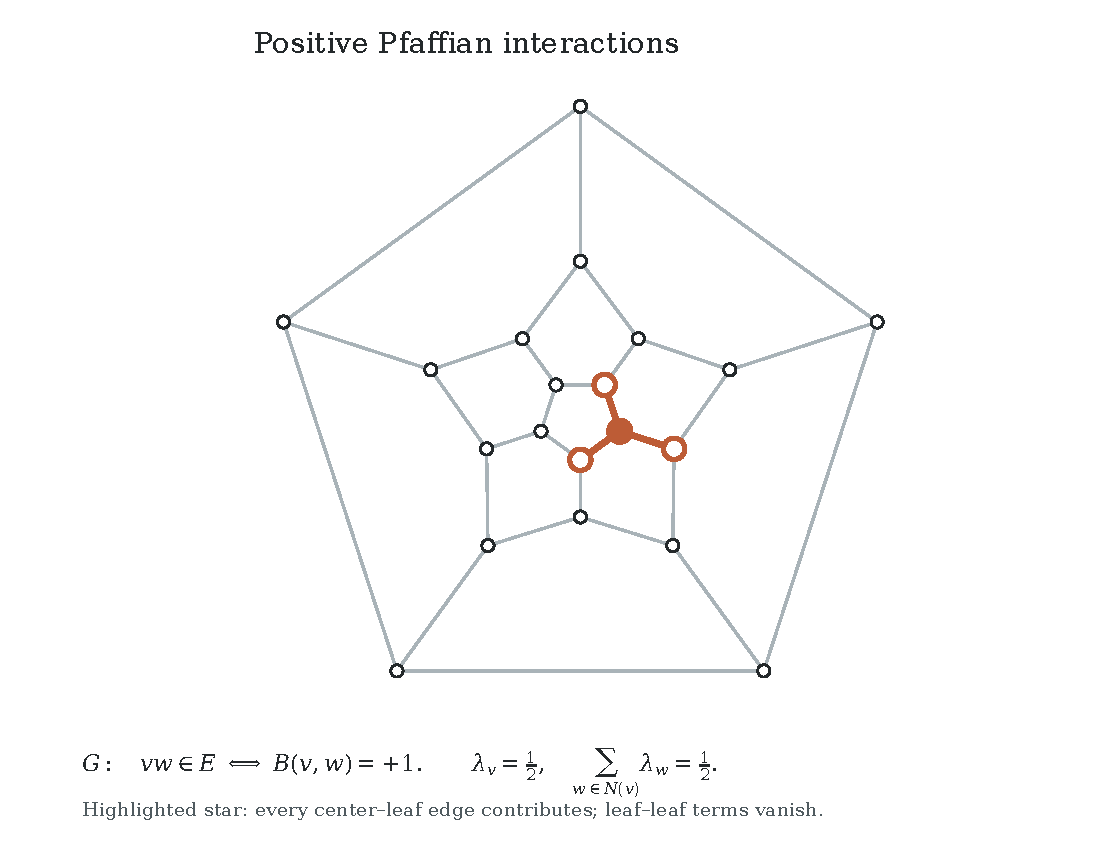
\includegraphics[width=.83\linewidth]{figures/pfaffian-graph.pdf}
 \caption{The positive-interaction graph on signed rank-two vertices.
 The highlighted star shows an equality support: half the mass is at its
 center and half is distributed among its three neighbors.}
 \label{fig:pfaffian-graph}
\end{figure}

\begin{proposition}\label{prop:simplex-equality-locus}
The set $\{z:S(z)=1,\ q(z)=1/4\}$ is exactly
\[
 \bigcup_{v\in\mathcal V}
 \left(\frac12v+\frac12\operatorname{conv}N_G(v)\right).
\]
Each $N_G(v)$ consists of three vertices, so this is a union of twenty
closed triangles. Negative-Pfaffian equality is obtained by any odd
coordinate permutation, and positive scaling gives all nonzero equality
forms.
\end{proposition}
\begin{proof}
Suppose $q(z)=1/4$ and choose a convex decomposition
$z=\sum_v\lambda_vv$. Both inequalities in the preceding proof are
equalities. The weights maximize the graph quadratic at $1/4$.
On their positive support, first-order variations show that all weighted
neighbor sums are equal. Their weighted average is twice the objective,
so each is $1/2$.

Choose a supported edge $uv$. The supported neighbor sets of $u$ and $v$
are disjoint, by triangle-freeness, and each has mass $1/2$. They therefore
partition the support. Each side is independent. Every vertex must be
adjacent to the whole opposite side, since its weighted degree is $1/2$
and every supported weight is positive. The support is complete
bipartite. The absence of four-cycles forces one side to be a singleton:
the support is a star, its center has mass $1/2$, and its leaves have total
mass $1/2$.

Conversely, any two neighbors of a vertex have underlying pairs in the
same remaining three-element set. They intersect, so their interaction
$B$ is zero. Every such balanced star therefore has Pfaffian $1/4$.
It lies in $C$; the proved inequality forces $S=1$.
\end{proof}

For example, the positive neighbors of $e_{12}$ are
\[
 e_{34},\qquad e_{13}-e_{14}+e_{34},\qquad
 e_{23}-e_{24}+e_{34}.
\]
Doubling this equality triangle gives the explicit family
\[
 \Omega=e_{12}+e_{34}
       +\mu(e_{13}-e_{14})+\nu(e_{23}-e_{24}),
 \qquad \mu,\nu\ge0,\quad\mu+\nu\le1,
\]
with $q(\Omega)=1$ and $S(\Omega)=2$. The union in the proposition is the
complete equality classification in pairing coordinates.

To pass from twenty triangles to the family in the theorem, relabel the
five barycentric gradients. If $B_\pi$ expresses the new four-vector basis
in the old one, the induced action is
$\Omega\mapsto B_\pi^T\Omega B_\pi$. It preserves $S$, and
$\det B_\pi=\operatorname{sgn}\pi$. An odd relabeling first makes the
Pfaffian positive. The even relabelings act transitively on $\mathcal V$:
even permutations fixing the omitted label give all twelve signed
coordinate vectors from $e_{12}$; exchanging the omitted label with a
third index, and exchanging the first two indices to preserve parity,
gives the eight signed triangle vectors. They therefore take any
equality triangle to the displayed one. Scaling then sets $q=1$.

For an explicit realization, let $X$ have columns
\[
 e_1,\ e_2,\ -\nu e_1+\mu e_2+e_3,\
 \nu e_1-\mu e_2+e_4.
\]
Then $X^T JX$ is the displayed $\Omega$, and $X^{-T}$ has columns
$(1,0,\nu,-\nu)$, $(0,1,-\mu,\mu)$, $e_3$, $e_4$.
The negative barycentric gradients of $K_{\mu,\nu}$ are the negatives
of the columns of $X$, together with their opposite sum. Hence this
simplex has the required pairing matrix. It has volume $1/24$ and
capacity $1/4$. Equal pairing matrices give affine symplectomorphisms,
so every equality simplex has the stated form up to the claimed
transformations.

The parameter boundary has a geometric meaning. The ten pairings of the
five weighted facet normals have absolute values
$1,1,1,1,\mu,\mu,\nu,\nu,1-\mu-\nu,1-\mu-\nu$.
An intersection of two facets is Lagrangian exactly when their normal
pairing vanishes. Thus interior parameters give equality simplices with
no Lagrangian two-faces, open edges give two, and the three corners give
four. Thus the equality family contains simplices with no Lagrangian
two-faces, as observed experimentally by Chaidez and Hutchings.

% Local certificate used in the global theorem in sixdim-global.tex.
% Requires theorem/lemma/proposition and standard amsmath/amssymb macros.
\section{A six-dimensional simplex and a hypergraph Lagrangian}
\label{sec:sixdim-hypergraph}

In dimension six, the standard simplex no longer maximizes the systolic
ratio, as Haim--Kislev observed numerically in her 2019 thesis
\cite[Remark~1.3]{HaimKislev2019CubesSimplices}. The pairing formulation gives a particularly simple exact example
and explains a numerical optimizer through a classical hypergraph
Lagrangian. We prove that the example is a strict local maximum among simplices,
modulo the natural symmetries; Section~\ref{sec:sixdim-global} proves it is
globally optimal and classifies equality.

For an alternating $6\times6$ matrix $\Omega$, put
\[
 S_6(\Omega)=\max_{\sigma\in\mathfrak S_6}
             \sum_{i<j}\Omega_{\sigma(i),\sigma(j)},\qquad
 C_6=\{\Omega:S_6(\Omega)\le1\}.
\]
The same barycentric-gradient argument as in the preceding section gives
\begin{equation}\label{eq:sixdim-simplex-ratio}
 \frac{c_{\mathrm{EHZ}}(K)^3}{6\operatorname{vol}_6K}
 =\frac{15|\operatorname{Pf}\Omega|}{S_6(\Omega)^3}
\end{equation}
for every six-simplex. Indeed the capacity is $1/(2S_6)$ and the volume
is $1/(6!|\operatorname{Pf}\Omega|)$. Every nondegenerate alternating
$\Omega$ occurs, and identical pairings determine labeled simplices up
to affine symplectomorphism.

Write $e_{ij}$ for an alternating coordinate vector and
$t_{ijk}=e_{ij}-e_{ik}+e_{jk}$ for $i<j<k$. Consider the five forms
\begin{equation}\label{eq:sixdim-five-vertices}
 v_1=t_{135},\qquad v_2=-t_{246},\qquad
 v_3=e_{12},\qquad v_4=e_{34},\qquad v_5=e_{56}.
\end{equation}
Each has $S_6(v_i)=1$: a coordinate order score is $\pm1$, as is the
score on an oriented triangle. The order $(1,3,5,2,6,4)$ has score $1$
on all five. Consequently $S_6=1$ on their entire convex hull.

\begin{theorem}\label{thm:sixdim-golden-local}
Let
\[
 a=\frac{13+3\sqrt5}{62},\qquad b=\frac{6-\sqrt5}{31},\qquad
 \Omega_*=a(t_{135}-t_{246})+b(e_{12}+e_{34}+e_{56}).
\]
Then $S_6(\Omega_*)=1$ and
\[
 \operatorname{Pf}\Omega_* =\frac{63+5\sqrt5}{1922}.
\]
The corresponding six-simplex has systolic ratio
\[
 \frac{945+75\sqrt5}{1922}>\frac59,
\]
strictly exceeding the standard simplex's ratio. It is a strict local
maximum among six-simplices modulo translations, positive dilations
and linear symplectomorphisms.
\end{theorem}

The value is approximately $0.5789308524$; its cube root is approximately
$0.8334423504$. Leipold reports the nearby root-normalized numerical value
$0.8334409621$~\cite[Section~12.4 and Appendix]{Leipold2026}. Numerical
proximity alone does not identify the two simplex configurations. The
exact proof here establishes this candidate's global optimality below.

\subsection{The five-vertex face and its cubic}

Direct Pfaffian expansion gives
\begin{equation}\label{eq:sixdim-F32}
 \operatorname{Pf}(xv_1+yv_2+zv_3+uv_4+vv_5)
 =xy(z+u+v)+zuv.
\end{equation}
Here the scalar variable $v$ in the right-hand side is distinct from the
indexed forms $v_i$. This is the edge polynomial of the $3$-uniform
hypergraph
\[
 F_{3,2}=\{123,124,125,345\}.
\]
Its Lagrangian and maximizing weights are classical: Baber and Talbot
record exactly these weights and the value
$(189+15\sqrt5)/961$ with their normalization, which is six times the
polynomial in~\eqref{eq:sixdim-F32}~\cite[Theorem~22]{BaberTalbot2012}.
Thus the symplectic ratio in Theorem~\ref{thm:sixdim-golden-local} is
$5/2$ times that hypergraph Lagrangian. We include the short maximization
argument to keep the geometric result independent of any extremal
hypergraph theorem.

For nonnegative weights summing to one, put $t=z+u+v$. The arithmetic--
geometric mean inequality gives
\[
 xy(z+u+v)+zuv
 \le \frac{(1-t)^2t}{4}+\frac{t^3}{27}
 =:G(t),\qquad 0\le t\le1.
\]
Equality requires $x=y=(1-t)/2$ and $z=u=v=t/3$, apart from irrelevant
zero-mass endpoint cases. Comparing the endpoints and the two critical
points of
\[
 G(t)=\frac t4-\frac{t^2}{2}+\frac{31t^3}{108}
\]
gives its unique maximum at
$t_*=(18-3\sqrt5)/31$. This is precisely the stated pair of weights
$a,b$. Moreover the restricted Hessian is negative definite. To see this,
write $x=(1-t)/2+\delta$, $y=(1-t)/2-\delta$, and
$(z,u,v)=(t/3+\eta_1,t/3+\eta_2,t/3+\eta_3)$ with
$\sum\eta_i=0$. The polynomial becomes
\[
 G(t)-t\delta^2-\frac t6\sum_i\eta_i^2+\eta_1\eta_2\eta_3.
\]
At $t=t_*$, $G''(t_*)=-\sqrt5/6<0$; the other quadratic terms are
strictly negative on the three remaining tangent directions.

We next verify that this weight simplex is an actual face of the full
fifteen-dimensional polytope $C_6$. This point matters: optimization on
five chosen generators alone would not imply local maximality under
arbitrary affine deformations.

For an order $\sigma$, let $p_\sigma$ be its fifteen-coordinate sign
vector. Let $\tau=(1\,3\,5)(2\,4\,6)$ act on the labels of an order.
Let $\mathcal I$ consist of the three cyclic images under $\tau$ of each
of the following seven orders:
\begin{equation}\label{eq:sixdim-active-orders}
 \begin{array}{cccc}
 123564,&132564,&134256,&134526,\\
 135264,&135426,&135642.&
 \end{array}
\end{equation}
These are exactly the twenty-one orders having score $1$ on all five
forms in~\eqref{eq:sixdim-five-vertices}. Their common affine equality
set $p_\sigma\cdot\Omega=1$ is four-dimensional. More explicitly,
subtracting the displayed equations gives
\[
 \begin{gathered}
 \Omega_{14}=\Omega_{16}=\Omega_{23}=\Omega_{25}
 =\Omega_{36}=\Omega_{45}=0,\\
 \Omega_{13}=\Omega_{35}=-\Omega_{15},\qquad
 \Omega_{24}=\Omega_{46}=-\Omega_{26},\\
 \Omega_{13}-\Omega_{24}+\Omega_{12}+\Omega_{34}+\Omega_{56}=1.
 \end{gathered}
\]
These are eleven independent affine equations and identify the equality
set with $\sum_{i=1}^5\lambda_i v_i$, $\sum_i\lambda_i=1$.
For $i=1,\ldots,5$, respectively, the orders
\[
 125364,\quad123456,\quad213564,\quad142356,\quad123645
\]
have score $-1$ on $v_i$ and score $1$ on the other four forms. Their
inequalities read $1-2\lambda_i\le1$, forcing $\lambda_i\ge0$.
It follows that the common face is exactly
$F=\operatorname{conv}\{v_1,\ldots,v_5\}$.

\subsection{A certificate against every transverse affine deformation}

Set $q(\Omega)=\operatorname{Pf}\Omega$. Let $\mathcal J$ be the
three cyclic images of the distinguished order $135264$ in
\eqref{eq:sixdim-active-orders}. Differentiating the Pfaffian at
$\Omega_*$ gives the exact identity
\begin{equation}\label{eq:sixdim-gradient-certificate}
 \nabla q(\Omega_*)
 =\alpha\sum_{\sigma\in\mathcal I\setminus\mathcal J}p_\sigma
  +\beta\sum_{\sigma\in\mathcal J}p_\sigma,
 \quad
 \alpha=\frac{41-12\sqrt5}{5766}>0,
 \quad\beta=\frac{-19+29\sqrt5}{1922}>0.
\end{equation}
This is a fifteen-coordinate identity over $\mathbb Q(\sqrt5)$; the
explicit orders and coefficients give a small independently checkable
certificate.

For every feasible displacement $h$ from $\Omega_*$, each active order
satisfies $p_\sigma\cdot h\le0$. The positivity in
\eqref{eq:sixdim-gradient-certificate} implies
$\nabla q(\Omega_*)\cdot h\le0$, with equality precisely when $h$ lies
in the tangent space of $F$. On that tangent space, the Hessian is
negative definite by the preceding computation.

These two facts imply strict local maximality on $C_6$. Indeed, if
nonzero feasible displacements $h_k\to0$ satisfied
$q(\Omega_*+h_k)\ge q(\Omega_*)$, pass to a convergent subsequence of
$h_k/\|h_k\|$, with unit limit $d$. Taylor expansion first forces
$\nabla q(\Omega_*)\cdot d=0$, so $d$ belongs to the face tangent
space. The Hessian is strictly negative in direction $d$. The linear
term is nonpositive for every $h_k$, so the second-order Taylor expansion
now gives a strict decrease for large $k$, a contradiction.

Finally, radial normalization by $S_6$ identifies nearby nondegenerate
pairing forms, modulo dilation, with a neighborhood in the boundary of
$C_6$. Formula~\eqref{eq:sixdim-simplex-ratio} transfers the strict
local Pfaffian maximum to the stated strict local systolic maximum,
modulo affine symplectomorphisms and translations. This proves
Theorem~\ref{thm:sixdim-golden-local}.

The local certificate uses no complete facet enumeration of the
linear-ordering polytope. The global proof in the next section uses an
exact computer-assisted vertex classification. The contrast with
dimension four is structural: a quadratic graph
optimization is replaced by a cubic hypergraph optimization, and the
hypergraph $F_{3,2}$ already appears using only coordinate and triangle
forms.

% Global extension, independently mathematically audited 2026-10-28.
% Exact polyhedral classification is computer-assisted; see retained verifier.
\section{The sharp global six-simplex inequality}
\label{sec:sixdim-global}

The local example from Theorem~\ref{thm:sixdim-golden-local} is in fact
optimal among all six-simplices. The proof combines a small hypergraph
argument with an exact finite description of a linear-ordering relaxation.
The finite description is independently reproduced with two exact polyhedral
backends; the inequalities used after that description are explicit.

\begin{theorem}\label{thm:sixdim-global}
Every six-dimensional simplex $K$ satisfies
\[
 \frac{c_{\mathrm{EHZ}}(K)^3}{6\operatorname{vol}_6K}
 \le \frac{945+75\sqrt5}{1922}.
\]
Equality holds precisely for the simplex in
Theorem~\ref{thm:sixdim-golden-local}, up to translation, positive homothety,
and linear symplectomorphism.
\end{theorem}

Put $q_*=(63+5\sqrt5)/1922$. By
\eqref{eq:sixdim-simplex-ratio}, it suffices to maximize
$|\operatorname{Pf}\Omega|$ on $C_6$. Let
\[
 D_6=\operatorname{conv}\bigl(\{\pm e_{ij}:1\le i<j\le6\}
       \cup\{\pm t_{ijk}:1\le i<j<k\le6\}\bigr),
\]
so $D_6$ has
seventy rank-two generators and is contained in $C_6$.

\subsection{The rank-two hull}

Introduce seven points $u_1,\ldots,u_6,u_7$ with $u_i=e_i$ for $i\le6$
and $u_7=0$. For each three-element set $T=\{i,j,k\}$, choose the form
\[
 b_T=(u_i-u_k)\wedge(u_j-u_k).
\]
Then $D_6=\operatorname{conv}\{\pm b_T\}$. The orientation choices will
not matter for an upper bound. If two triples share two labels, their forms
share a wedge factor, so $b_T\wedge b_U=0$. Also $b_T\wedge b_T=0$.
Consequently the Pfaffian cubic in coefficients of these forms is
multiaffine, and contains no monomial involving both $T$ and $U$ when
$|T\cap U|\ge2$.

Cancel antipodal coefficients in a convex decomposition. It becomes
$\Omega=\sum_Td_Tb_T$ with $\sum_T|d_T|\le1$. Homogeneity permits a
nonzero global maximizer to be chosen with total mass one. Among global
maximizers choose one with smallest support. If two supported types share
two labels, fix their signs and their total absolute mass, and vary the
split between them. The Pfaffian is affine in that split. Its absolute
value therefore attains a maximum at an endpoint, removing one supported
type without lowering the objective. This contradicts minimality. Thus
some global maximum is supported on a family of triples whose pairwise
intersections have size at most one.

We record the elementary classification needed here. A maximal such family
on seven labels has either five or seven triples. Indeed, each triple uses
three of the twenty-one label pairs, so there are at most seven triples.
No label can have degree zero: otherwise maximality requires all pairs on
the other six labels to be covered, which would give degree $5/2$ at each
of those labels. If a label has degree one, with its only triple $vab$,
all six pairs among the remaining four labels $R$ must be covered.
Without a triple contained in $R$, this requires six additional triples,
forcing all twenty-one pairs to be covered and contradicting degree one.
With a triple $xyz\subset R$, the three pairs $wx,wy,wz$, where
$R=\{w,x,y,z\}$, require three separate triples using $a$ or $b$.
One of the pairs $wa,wb$ would then repeat. Hence every label has degree
at least two, and there are at least five triples. Six triples would leave
three uncovered pairs with even degree at every label, hence an uncovered
triangle, contradicting maximality.

With five triples the degree sequence is $(3,2,2,2,2,2,2)$. The three
triples through the degree-three label match the other six labels. The two
remaining triples partition those six labels, and each matching pair crosses
that partition. Up to relabeling this is
\[
 \{135,246,127,347,567\}.
\]
With seven triples every label pair is covered exactly once: the family is
the Fano plane.

For three members of a linear triple family, the Pfaffian coefficient is
zero if their union has at most six labels, since the forms lie in a
difference space of dimension at most five. When their union has seven
labels, their six edge factors form a spanning tree and the coefficient is
$\pm1$. For the five-triple configuration, taking absolute values therefore
gives the polynomial
\[
 xy(z+u+v)+zuv.
\]
Its maximum under nonnegative total mass one is $q_*$, as computed in
\eqref{eq:sixdim-F32}. For the Fano configuration the unsigned polynomial
is the Fano-plane Lagrangian, because the nonzero triples are precisely
three concurrent Fano lines.

Here is a short bound for the latter polynomial $P$. On the boundary,
remove a zero-weight point. The four remaining Fano triples are transversal
to a partition of the six remaining points into three pairs. Hence $P$ is
at most the product of the three class masses, and is at most $1/27$.
At a full-support maximum, the seven partial derivatives all equal $3P$.
Their sum counts every pair exactly once, giving
\[
 21P=\sum_{i<j}x_ix_j\le\frac37,
 \qquad P\le\frac1{49}.
\]
Thus $P\le1/27<q_*$. Together with the explicit attaining example, this
proves
\begin{equation}\label{eq:sixdim-ranktwo-bound}
 \max_{\Omega\in D_6}|\operatorname{Pf}\Omega|=q_*.
\end{equation}

\subsection{The finite polyhedral decomposition}

All pairings in this subsection use the fifteen upper-triangular entries.
Define
\[
 F=\frac15\begin{pmatrix}0&M\\-M^T&0\end{pmatrix},
 \quad M=2I-\mathbf1\mathbf1^T,
 \qquad
 p_0=\begin{pmatrix}0&N\\-N^T&0\end{pmatrix},
 \quad N=I-\mathbf1\mathbf1^T.
\]
The form $F$ is a normalized three-fence. Let $\mathcal F$ be its orbit
under the seven-label permutation action. The action on forms comes from
relabeling the seven barycentric gradients and has determinant $\pm1$;
it preserves $C_6$, $D_6$ and the absolute Pfaffian. Its dual action on
functionals is contragredient.

The retained replay in
\path{certificates/sixdim-global/README.md} specifies four small programs:
\begin{center}
\begin{tabular}{ll}
\path{algebra.py} & \path{local_maximum.py}\\
\path{full_classification.py} & \path{dual_coverage.py}
\end{tabular}
\end{center}
The latter two use exact cdd and PPL polyhedral backends. Their generated
outputs and a fresh copied-package run receipt are retained beside the
programs. This is a computer-assisted completeness check, not a formalized
proof in a proof assistant.

The exact finite calculations establish the following facts:
\begin{enumerate}
\item $Q_6=D_6^\circ$ has exactly $1560$ vertices: the $720$ order
functionals and the $840$ elements of the dual orbit of $p_0$.
\item $\mathcal F$ has $840$ elements. The canonical pairing is
$p_0\cdot F=6/5$, whereas $p_0\cdot F'\le4/5$ for every other
$F'\in\mathcal F$. Every fence satisfies every order inequality.
\item The vertex $p_0$ has eighteen neighbors in $Q_6$, all order
functionals. They are exactly the eighteen orders with $F\cdot p=1$.
The face $B=\{X\in D_6:p_0\cdot X=1\}$ has eighteen rank-two vertices
and affine dimension fourteen.
\end{enumerate}

For completeness, the completeness check in the first item uses graph
connectivity, not a sample of vertices. Six adjacent-transposition generators
preserve the seventy inequalities of $Q_6$ and generate the two disjoint
orbits. At an order representative, both exact polyhedral backends give
$186$ extreme tangent rays, whose exact endpoints are $165$ order vertices
and $21$ fractional vertices. At $p_0$ they give eighteen rays, all with
order endpoints. Both representatives have active rank fifteen. The candidate
set is therefore closed under every neighbor in the one-skeleton. Since a
bounded polytope has connected one-skeleton, there are no further vertices.

Cut $Q_6$ by the $840$ inequalities $F'\cdot p\le1$. Each cut removes
its corresponding fractional vertex and meets all its incident edges at
existing integral neighbors. This can be done sequentially without creating
vertices: all other fractional vertices lie strictly inside the current cut,
so their tangent cones are unchanged; their original edges to integral
neighbors remain feasible in full. Thus each later cut has the same crossing
edges and introduces no new endpoint. The resulting polytope is precisely
the convex hull of the order functionals. Polarity gives
\[
 C_6=\operatorname{conv}(D_6\cup\mathcal F).
\]

Moreover, the midpoint of any two distinct fences lies in $D_6$. On an
order functional both endpoint scores are at most one; on a fractional
functional at most one is $6/5$, while the other is at most $4/5$.
Replacing equal masses of two fences by their midpoint repeatedly reduces
any convex combination to a point of $D_6$ or a combination of $D_6$ and
one fence. Each fence violates exactly one facet inequality of $D_6$.
Consequently $C_6$ is covered by $D_6$ and the $840$ pyramids
$\operatorname{conv}(F',B_{F'})$. It remains to bound one pyramid.

\subsection{A quadratic bound on a fence pyramid}

Write $X=\sum_{i=1}^{18}x_iv_i\in B$, with $x_i\ge0$ and
$\sum_i x_i=1$. Exact Pfaffian expansion gives
\[
 \operatorname{Pf}(tF+sX)
 =\frac4{125}t^3+\frac2{25}t^2s+Q(X)ts^2
       +\operatorname{Pf}(X)s^3.
\]
Here $Q(X)=x^THx/10$, where $H$ is a symmetric integer matrix with zero
diagonal and entries $0,1,2$. The graph of entries equal to two is the
disjoint union of six three-vertex paths. In each path, the two leaves have
entry zero between them; entries between distinct paths are zero or one.
These explicit coefficient properties give
\[
 \mathbf1\mathbf1^T-H
 =\sum_{\text{six paths }(c,l,r)}
       (e_c-e_l-e_r)(e_c-e_l-e_r)^T+R,
 \qquad R\ge0\ \text{entrywise}.
\]
Hence $0\le Q(X)\le1/10$. By~\eqref{eq:sixdim-ranktwo-bound}, for
$t,s\ge0$,
\[
 |\operatorname{Pf}(tF+sX)|
 \le\frac4{125}t^3+\frac2{25}t^2s+\frac1{10}ts^2+q_*s^3
 \le q_*(t+s)^3.
\]
The last inequality is strict when $t>0$, because $q_*>1/30$.
This proves the global bound, with strictness outside $D_6$.

\subsection{Equality}

Begin with any global maximizer in $D_6$ and apply the signed mass-merging
procedure. At each interior split, the absolute value of an affine function
already has its global maximum; that affine function must be constant.
Thus the procedure gives a finite path of global maximizers to a supported
linear triple packing. The Fano case is too small. In the five-triple case,
equality forces the golden weights and common signs for the two central
variables and for the three outer variables. All four resulting sign
patterns are relabelings of $\Omega_*$: $(1\,3)(2\,4)$ flips the two
triangle signs, and $(1\,2)(3\,4)(5\,6)$ negates the entire form.

Every endpoint is therefore a strict local maximum on $C_6$, by
Theorem~\ref{thm:sixdim-golden-local}. A nonconstant segment of global
maximizers cannot end at such a point. Working backward through the finite
merging path shows that the original form was the same endpoint. Thus every
maximizer is a seven-label relabeling of $\Omega_*$. Identical normalized
barycentric-gradient pairings determine simplices up to affine
symplectomorphism, proving the equality statement in
Theorem~\ref{thm:sixdim-global}.

\section{A sharp difference-area inequality for squared bodies}
\label{sec:squared}
Let $\sigma:\mathbb C\to\mathbb C$ be $\sigma(z)=z^2$. We prove
\[
 \area(\sigma K-\sigma K)\leq5\area(\sigma K)
\]
for every origin-symmetric planar convex body $K$, with a sharp constant.
The proof identifies squared bodies with planar reciprocal bodies, reduces
arbitrary sources to parallelograms, and bounds their squares by a geometric
argument valid in every dimension. The last argument gives a sharp
supremum for intersections of two confocal paraboloids; it does not bound
arbitrary higher-dimensional reciprocal bodies.

For a planar body $L$ write
\[
 R(L)=\frac{\area(L-L)}{4\area(L)}.
\]
This quotient is invariant under invertible affine maps. The planar bound
is $R\leq5/4$. Through the quaternionic construction of
Chaidez--Tanny~\cite{CT2026}, it bounds $c_{\EHZ}(X)^2$ by
$(5/2)\Vol_4(X)$ for bodies with right quaternionic $I$-symmetry.
We give the Finsler and capacity normalizations at the end of the section.
A \emph{source body} below is compact, origin-symmetric, convex, and has
nonempty interior.

\subsection{Complex squaring and reciprocal convexity}
Following Milman--Milman--Rotem~\cite{MMR2018}, write
\[
 M'=\{y:\langle y,n\rangle\leq h_M(n)^{-1}\ \text{for all }n\in S^1\}.
\]
Their Lemma 18 and Proposition 19 express $M'$ as the intersection, over $x\in M$, of the parabolic regions
\[
 P_x=\{y:\langle y,x\rangle\leq 1-\tfrac14|x|^2|\operatorname{proj}_{x^\perp}y|^2\},\quad P_0=\mathbb R^2.
\]
For $x=re^{i\theta}$, elementary squaring gives
\[
 P_x=\sigma(S_x),\qquad S_x=\{z:|\operatorname{Re}(e^{-i\theta/2}z)|\leq r^{-1/2}\}.
\]
Indeed, in coordinates $e^{-i\theta}y=u+iv$, both descriptions are $u\leq r^{-1}-rv^2/4$. The map $\sigma$ commutes with arbitrary intersections of centrally symmetric sets: the two square roots of a point either both belong to any such set or both fail to belong.

\begin{theorem}[Squared bodies and reciprocity]
The compact planar reciprocal bodies containing the origin in their interior are precisely the images $\sigma(K)$ of source bodies. Moreover,
\[
 (\sigma K)'=\sigma(K^\circ).
\]
\end{theorem}
\begin{proof}
Write $K$ as the intersection of its symmetric supporting strips with unit normals $n=e^{i\phi}$ and half-widths $h_K(n)$. Each strip maps to $P_{x_\phi}$, where $x_\phi=e^{2i\phi}/h_K(n)^2$. Consequently $\sigma K$ is convex. Since $n/h_K(n)$ runs over $\partial K^\circ$, the points $x_\phi$ run over $\partial\sigma(K^\circ)$. This last image is also convex by the same strip argument. The parabolic representation therefore gives
\[
 \sigma K=(\sigma(K^\circ))'.
\]
Apply the same identity to $K^\circ$ to obtain the stated conjugacy. Conversely, the parabolic representation of any reciprocal $M'$ identifies it with $\sigma(\bigcap_{x\in M}S_x)$. The intersection is centrally symmetric and convex; compactness and interior of its square imply the corresponding properties of the intersection itself.
\end{proof}
This is an identity in fixed Euclidean coordinates. Neither squaring nor reciprocity is asserted to commute with arbitrary affine maps.

\subsection{Two confocal paraboloids in arbitrary dimension}

We first record the shadow-system fact used twice below. If points move
parallel to a fixed vector $e$ according to
\[
 C_t=\conv\{p+t\beta(p)e:p\in S\},
\]
then $\Vol_d(C_t)$ is convex in $t$. Indeed, the projection onto
$e^\perp$ is fixed. On each line parallel to $e$, the upper endpoint is
a supremum of affine functions of $t$, and the lower endpoint an infimum:
the admissible convex combinations are specified by their fixed transverse
coordinate. The fiber length is therefore convex, and integration proves
the assertion. If convex bodies $C_t$ are given by such moving points,
then $C_t-C_t$ is another shadow system, with generators $p-q$ and
velocities $\beta(p)-\beta(q)$.

\begin{theorem}[Two-paraboloid difference-volume bound]
\label{thm:two-paraboloids}
Let $d\geq2$, and let $Q\subset\mathbb R^d$ be a bounded intersection
of two solid paraboloids of revolution with a common focus. Then
\[
 \frac{\Vol_d(Q-Q)}{\Vol_d(Q)}<C_d,
 \qquad C_d=\frac{2^{d+1}(d-1)+2}{d}.
\]
The constant $C_d$ is the supremum over this class, and is approached by
an affine-normalized degeneration to the round parabolic cap
\[
 P_d=\{(u,z):0\leq u\leq1,\ |z|^2\leq u\}.
\]
\end{theorem}
\begin{proof}
\emph{Normalize the pair.}
Translate the common focus to the origin. The two inequalities are
\[
 |y|+a_i\cdot y\leq c_i,\qquad |a_i|=1,\quad c_i>0,
 \quad a_1\ne a_2.
\]
The last condition is necessary for boundedness. On the future light cone
$r=|y|$, the covectors $\ell_i=(1,a_i)/c_i$ are null for the quadratic
form $r^2-|y|^2$. Their sum is timelike, since
\[
 (\ell_1+\ell_2)_0^2-| (\ell_1+\ell_2)_{\mathrm{sp}}|^2
 =\frac{2(1-a_1\cdot a_2)}{c_1c_2}>0.
\]
A Lorentz transformation sends that sum to the time axis. The transformed
null covectors then have opposite spatial parts and equal positive time
coordinates. A common rescaling and a spatial rotation give the lens
\[
 L=\{(x,z):\sqrt{x^2+|z|^2}+|x|\leq1\}
   =\{(x,z):|x|\leq\tfrac12,\ |z|^2\leq1-2|x|\}.
\]
This change preserves the class: Lorentz maps preserve the future cone
and future null covectors, so each inequality remains a confocal
paraboloid inequality after division by its positive time coefficient.
A Lorentz transformation is a spatial rotation composed with a boost;
the latter has spatial part
$(y_1,y_\perp)\mapsto(\gamma(y_1+t|y|),y_\perp)$,
where $|t|<1$ and $\gamma=(1-t^2)^{-1/2}$.
Consequently, up to an invertible spatial linear map, every original
$Q$ is
\[
 T_v(L),\qquad T_v(y)=y+|y|v,\quad |v|<1.
\]
These images are convex by the same Lorentz calculation, and remain
convex for $|v|=1$ by Hausdorff continuity.

\emph{Enlarge the shadow family.}
Write $v=ca+b$, where $a$ is the $x$-axis and $b\perp a$. Define
\[
 F_{c,b}(x,z)=(x,z)-|x|(c,b).
\]
We claim that $F_{c,b}(L)$ is convex throughout the larger parameter set
$|c|\leq1$, $|b|\leq1$. For $|c|<1$, its positive and negative halves
are affine images of the half-lenses, on opposite sides of the common
interface $D=\{0\}\times B^{d-1}$. Take one point in either half:
\[
 Y_+=((1-c)t,z-tb),\qquad
 Y_-=(-(1+c)r,w-rb),
\]
where $t,r\geq0$, $|z|^2\leq1-2t$ and $|w|^2\leq1-2r$.
The segment crosses the interface at a point with transverse coordinate
\[
 z_0=\lambda z+(1-\lambda)w-[\lambda t+(1-\lambda)r]b
\]
for some $\lambda\in[0,1]$. Since
$\sqrt{1-2t}\leq1-t$ and likewise for $r$, we have $|z_0|\leq1$.
The crossing lies in $D$, so the whole segment lies in the union of the
two convex halves. This proves convexity; the endpoint values of $c$
follow by continuity.

On $\partial L$ we have $|y|=1-|x|$, and hence
$T_v(y)=v+F_{c,b}(y)$. For $|v|<1$, the map $T_v$ is a homeomorphism:
on each preserved transverse line, its coordinate along $v$ is strictly
increasing. Thus support maxima of $T_v(L)$ occur on $T_v(\partial L)$.
Support maxima of $F_{c,b}(L)$ occur on the two outer parabolic sheets
or the interface rim, also images of points of $\partial L$.
Equality of support functions gives
\[
 T_v(L)=v+F_{c,b}(L),\qquad |v|\leq1,
\]
with the unit-vector case obtained by continuity. This is equality of
image bodies; the maps need not agree at interior points.

The two affine half-maps have determinants $1-c$ and $1+c$.
Their interiors are disjoint and the original half-volumes equal, so
\[
 \Vol_d(F_{c,b}(L))=\Vol_d(L).
\]
For fixed $b$, varying $c$ moves all points parallel to $a$, with speed
$-|x|$. The difference-body volume is therefore convex in $c$, and its
quotient by volume is bounded by the larger quotient at $c=\pm1$.

\emph{Identify the endpoints.}
At $c=1$ the positive half collapses into $D$, because
$|z-tb|\leq|z|+t\leq1$. The negative half has coordinates
\[
 u=-2r,\qquad w=z-rb,\qquad |z|^2\leq1-2r.
\]
The affine change $U=1+u$, $Z=w-(u/2)b$ identifies it with $P_d$.
The other endpoint is its reflection. Writing $\omega_{d-1}$ for the
volume of the unit $(d-1)$-ball, we obtain
\[
 \Vol_d(P_d)=\frac{2\omega_{d-1}}{d+1},\qquad
 \Vol_d(P_d-P_d)=2\omega_{d-1}
   \int_0^1(1+\sqrt{1-s})^{d-1}\,ds.
\]
For fixed difference coordinate $s\geq0$, the transverse difference
balls increase as the source coordinate increases; the largest is
attained at the pair $1,1-s$. Evaluating the integral gives the stated
quotient $C_d$.

Finally, along the original radial shadow $T_{te}(L)$ the volume is
constant: its Jacobian is $1+t\langle e,y\rangle/|y|$, and the odd term
integrates to zero. The quotient at $t=0$ is $2^d<C_d$, whereas that at
$t=1$ is at most $C_d$. Convexity of the numerator gives strictness for
$|t|<1$. As $v\to a$, the images tend to a translate of $P_d$; volume
continuity proves sharpness of the supremum.
\end{proof}

\subsection{Endpoint caps and positive tent decompositions}
For a squared planar body $L$, let
\[
 T_t(u,v)=(u+t\sqrt{u^2+v^2},v),\qquad -1\leq t\leq1.
\]
For $|t|<1$, this is affine equivalent to another squared body, since
\[
 \sigma(\sqrt{1+t}\,x+i\sqrt{1-t}\,y)
 =\bigl(\operatorname{Re}\sigma z+t|\sigma z|,
         \sqrt{1-t^2}\operatorname{Im}\sigma z\bigr).
\]
The images are convex, including the endpoints by continuity. The
Jacobian gives
\[
 \area(T_tL)=A+tB,\qquad A=\area(L),\quad
 B=\int_L\frac{u}{\sqrt{u^2+v^2}}\,du\,dv,
 \qquad |B|<A.
\]
The difference bodies form a shadow system, so their areas are convex
in $t$. Dividing the endpoint interpolation by the positive affine
function $4(A+tB)$ proves
\[
 R(L)\leq\max\{R(T_{-1}L),R(T_1L)\}.
\]
Since $T_1(\sigma(x+iy))=(2x^2,2xy)$, it suffices to bound the caps
\[
 C_K=\{(x^2,xy):(x,y)\in K\}.
\]
The other endpoint is the same construction after exchanging source
coordinates.

Normalize the horizontal projection of $K$ to $[-1,1]$ and write
\[
 K=\{(x,y):-1\leq x\leq1,\ -b(-x)\leq y\leq b(x)\},
\]
where $b$ is concave. A source shear $y\mapsto y+cx$ induces the affine
cap shear $(u,v)\mapsto(u,v+cu)$. Choose it so that
$b(-1)=b(1)=d\geq0$; then $b\geq d$. The cap sections are
\[
 -V_b(u)\leq v\leq U_b(u),\quad
 U_b(u)=\sqrt u\,b(\sqrt u),\quad
 V_b(u)=\sqrt u\,b(-\sqrt u),\qquad 0\leq u\leq1.
\]
Their area $A(b)=\int_0^1(U_b+V_b)$ is linear in $b$. Define
\[
 \begin{aligned}
 H_+(b,s)&=\max_{0\leq u\leq1-s}
               [U_b(u+s)+V_b(u)],\\
 H_-(b,s)&=\max_{0\leq u\leq1-s}
               [V_b(u+s)+U_b(u)].
 \end{aligned}
\]
The upper and lower endpoints of each difference section give
\[
 N(b):=\area(C_b-C_b)
      =2\int_0^1[H_+(b,s)+H_-(b,s)]\,ds.
\]
Each maximum is positively homogeneous and convex in $b$; thus $N$ is
subadditive.

For $-1<a<1$, let
\[
 f_a(x)=\begin{cases}
 (1+x)/(1+a),&x\leq a,\\
 (1-x)/(1-a),&x\geq a.
 \end{cases}
\]
Every continuous concave profile with equal endpoints is a uniform limit
of positive combinations of $1$ and these tents. For piecewise-linear
profiles this follows by matching their slope jumps; uniform concave
piecewise-linear approximation gives the general case. By linearity of
$A$ and subadditivity of $N$, it therefore suffices to prove $N\leq5A$
for the constant profile and for each single tent.

\begin{figure}[tb]
 \centering
 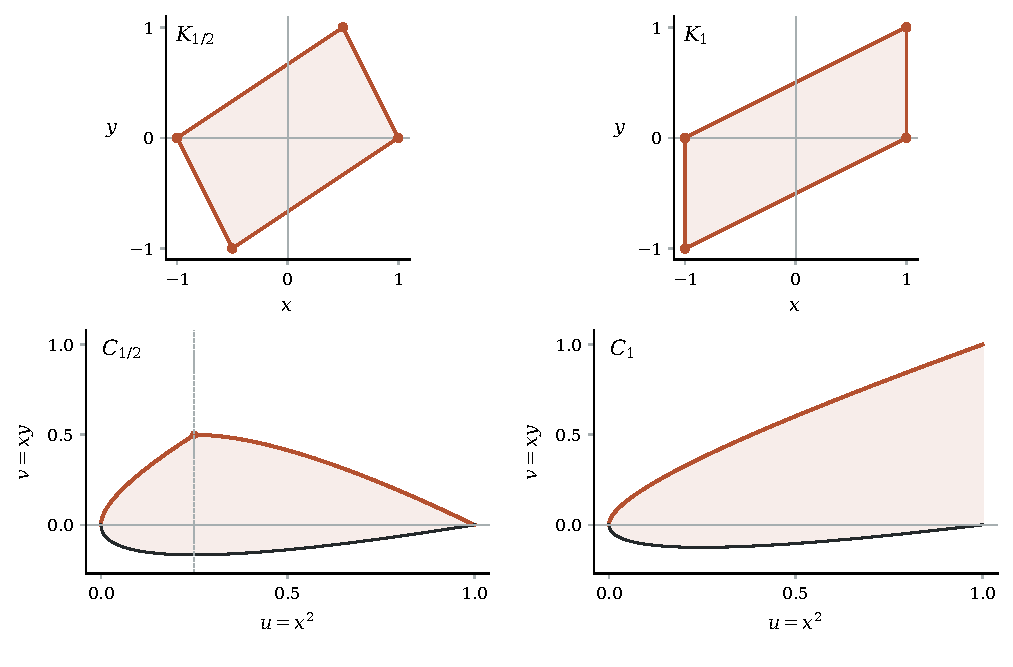
\includegraphics[width=.90\linewidth]{figures/tent-caps-compact.pdf}
 \caption{A single-tent source is a parallelogram. Its cap is a limit of
 affine-normalized squares of flattened parallelograms, so the
 two-paraboloid theorem applies without evaluating the difference-area
 integral.}
 \label{fig:tent-caps}
\end{figure}

\begin{theorem}[Sharp planar difference-area bound]
\label{thm:squared-five}
For every origin-symmetric planar convex body $K$,
\[
 \area(\sigma K-\sigma K)\leq5\area(\sigma K).
\]
The constant five cannot be decreased. The same inequality holds for
all planar reciprocal bodies and their affine images.
\end{theorem}
\begin{proof}
The source of $f_a$ is the parallelogram
\[
 K_a=\conv\{(-1,0),(a,1),(1,0),(-a,-1)\};
\]
the constant profile has a rectangular source. Each is an intersection
of two symmetric strips, so its square is the intersection of two solid
confocal parabolas. Any invertible flattening remains a parallelogram.
Theorem~\ref{thm:two-paraboloids} with $d=2$ bounds the difference-area
quotient of each flattened square by five. After affine normalization,
these squares tend to the corresponding cap; positive limiting area and
Hausdorff continuity pass the bound to that cap. The positive-profile
reduction and then the endpoint reduction prove the inequality.

For sharpness, take $K_\epsilon=[-1,1]\times[-\epsilon,\epsilon]$.
Under $(u,v)\mapsto(u,v/(2\epsilon))$, its square tends to
$P_2=\{0\leq u\leq1,\ |v|\leq\sqrt u\}$, whose difference area is
five times its area. Reciprocity and affine invariance give the remaining
statements. Lower-dimensional sources follow by approximation.
\end{proof}

\subsection{Finsler and symplectic consequences}

We give the normalization in the transfer explicitly. For a Finsler metric
$F$ on $\mathbb{RP}^2$, let $\ell(F)$ be its shortest noncontractible
closed-geodesic length, and put
\[
 \mathcal V(F)=\int_{D_F^*\mathbb{RP}^2}\frac{\omega_{\mathrm{can}}^2}{2}.
\]
This is the unnormalized cotangent volume used by Chaidez--Tanny; it is
$\pi$ times the usual normalized Holmes--Thompson area. Let
$\overline F(v)=(F(v)+F(-v))/2$. Its unit codisks are
$(D_x^*F-D_x^*F)/2$, because the support function of this Minkowski average
is the average of the two tangent norms. The sharp planar theorem therefore gives
\[
 \mathcal V(\overline F)\leq\frac54\mathcal V(F)
\]
whenever all the unit codisks of $F$ are affine images of squared bodies.

\begin{corollary}\label{cor:squared-finsler}
For such a Finsler metric on $\mathbb{RP}^2$,
\[
 \ell(F)^2\leq\frac58\mathcal V(F).
\]
\end{corollary}
\begin{proof}
For any noncontractible loop, at least one of its two orientations has
$F$-length at most its $\overline F$-length. Thus
$\ell(F)\leq\ell(\overline F)$. The reversible Ivanov--Pu inequality,
in the normalization above, is
$\ell(\overline F)^2\leq\mathcal V(\overline F)/2$;
see \cite[Theorem~3.7 and Lemma~3.8]{CT2026}. Combine these inequalities.
\end{proof}

\begin{corollary}\label{cor:I-symmetric}
Let $X\subset\mathbb H$ be a full-dimensional convex body invariant
under right multiplication by the quaternion $I$, with the standard
symplectic structure in \cite{CT2026}. Then
\[
 c_{\EHZ}(X)^2\leq\frac52\Vol_4(X),\qquad
 \rho(X)\leq\frac54.
\]
\end{corollary}
\begin{proof}
First suppose $X$ is smooth and uniformly convex. The quaternionic
construction of Chaidez--Tanny associates a Finsler metric $F$ on
$\mathbb{RP}^2$ whose unit codisks are affine squared bodies. Their
four-sheet contact covering gives
\[
 c_{\EHZ}(X)\leq4\ell(F),\qquad
 \Vol_4(X)=4\mathcal V(F)
\]
(\cite[Theorem~4.4 and equations~(5.2)--(5.3)]{CT2026}). Hence
\[
 c_{\EHZ}(X)^2\leq16\ell(F)^2
 \leq10\mathcal V(F)=\frac52\Vol_4(X).
\]
For arbitrary convex $X$, use smooth uniformly convex approximants with
the same finite symmetry. One obtains them by smoothing the invariant
support function and adding a small Euclidean ball. Hausdorff continuity
of volume and of EHZ capacity passes the bound to $X$, as in
\cite[Remark~5.4]{CT2026}.
\end{proof}

The planar constant five is sharp; neither corollary asserts a sharp
constant for its geometric class. In particular the comparison between a
geodesic and its closed lift, and the compatibility of codisks coming from
one ambient body, may prevent simultaneous equality in the auxiliary
estimates. The corollary gives the explicit constant $\sqrt5/2$ in a setting where
\cite[Theorem~11]{CT2026} supplies an unspecified constant below $\sqrt{3/2}$ ; it does not
establish the Viterbo bound $\rho\leq1$ for $I$-invariant bodies.

% Integration fragment; uses amsmath, amssymb, amsthm.
% Source: Balitskiy--Mitrofanov--Polyanskii, arXiv:2603.12495v2
% (19 August 2026), Theorem 3.3, Section 6.2, Conjecture 6.1.
\section{Truncated parallelograms: strict Viterbo and competing covers}
\label{sec:truncated-square-cover}

Balitskiy, Mitrofanov and Polyanskii conjectured a particular optimal
trapezoidal partner for every square with one corner truncated
\cite[Section~6.2, Conjecture~6.1]{BMP2026}. We construct a different
trapezoidal partner which improves their proposed optimum on an open set
of truncation parameters. This disproves the optimizer assertion of that
conjecture. We first prove its strict-inequality assertion for every convex
partner, so the two assertions have different outcomes.

We use their normal-triangle covering theorem
\cite[Theorem~3.3]{BMP2026}: for a polygon $Q$, the inequality
$c_{\mathrm{EHZ}}(K\times_L Q)\geq1$ is equivalent to $K$ containing a
translate of each $Q$-normal triangle of unit $Q$-perimeter. Degenerate
triangles, namely segments traversed in both directions, are included.
The $Q$-perimeter of a closed polygonal curve with directed edge vectors
$e_i$ is $\sum_i h_Q(e_i)$, where $h_Q$ denotes the support function.
This quantity is unchanged by translating $Q$.

Choose
\[
 0<A,B<1,\qquad g=A+B-1>0,\qquad a=1-A,\qquad d=B-a^2.
\]
In particular $B>a$ and $d>0$. Put $r=g/B$ and $s=g/A$, and define
\[
 Q_{A,B}=\operatorname{conv}\{(0,0),(1,0),(1,1-r),(1-s,1),(0,1)\}.
\]
Both $r,s$ belong to $(0,1)$, so this is a genuine corner-truncated
square. Its area is
\begin{equation}\label{eq:truncated-Q-area}
 |Q_{A,B}|=1-\frac{rs}{2}=1-\frac{g^2}{2AB}.
\end{equation}

The outward-normal directions of $Q_{A,B}$ are
$\pm e_1,\pm e_2,(r,s)$. The only nondegenerate positively dependent
triple is $-e_1,-e_2,(r,s)$; the only minimal positive pairs are the two
opposite coordinate pairs. Consequently its complete list of unit normal
templates, up to translation, consists of
\begin{equation}\label{eq:four-truncated-templates}
 T=\operatorname{conv}\{(0,0),(A,0),(A,B)\},\quad -T,\quad
 H=[0,e_1],\quad V=[0,e_2].
\end{equation}
For completeness, traverse $T$ in the order $(A,B),(A,0),(0,0)$.
Its edge directions are
\[ -e_2,\quad -e_1,\quad(r,s), \]
 and its $Q_{A,B}$-perimeter
is one: the first two support-function contributions vanish, while
$h_{Q_{A,B}}(A,B)=1$, because the cut line is
$rx+sy=r+s-rs=g/(AB)$ and $(A,B)=(AB/g)(r,s)$.
The two coordinate segments have unit perimeter because $Q_{A,B}$ has
unit width in both coordinate directions. Reversing the order of the three
edge directions gives the translation class $-T$.

% Insert after defining Q_{A,B} and its four templates, before the new cover.
% Uses the notation A,B,g and labels in truncated-square-section.tex.
\subsection{The Viterbo inequality for all partners}

The covering description also proves the Viterbo inequality for the entire
corner-truncated-square class, independently of which cover has minimum area.

\begin{theorem}\label{thm:truncated-global-viterbo}
Let $Q\subset\mathbb R^2$ be a parallelogram with one corner cut off by a
line meeting the interiors of its two adjacent sides. For every planar
convex body $K$ with nonempty interior,
\[
 c_{\mathrm{EHZ}}(K\times_L Q)^2<2|K|\,|Q|.
\]
In the normalization $Q=Q_{A,B}$ above, every capacity-one cover satisfies
\begin{equation}\label{eq:truncated-global-area}
 |K|>\frac{AB}{2AB-(A+B-1)^2}.
\end{equation}
Thus the strict-inequality assertion of \cite[Conjecture~6.1]{BMP2026}
holds, although its proposed optimizer will be disproved below.
\end{theorem}

\begin{proof}
An affine change in the $Q$-plane, paired with its inverse transpose in
the $K$-plane, reduces to $Q_{A,B}$ without changing the capacity or the
product of areas. Scaling $K$, we may assume its product capacity is one.
It therefore contains translated copies of the four templates
$T,-T,H,V$ from \eqref{eq:four-truncated-templates}.

First, this implies a lattice covering property. Put
\[
 \Lambda=A\mathbb Z e_1+B\mathbb Z e_2.
\]
Split every fundamental rectangle by its diagonal parallel to $(A,B)$.
The resulting triangulation has cells that are translates of $T$ or $-T$.
We use the triangulation-covering lemma
\cite[Lemma~4.3]{BMP2026}: if every cell of a planar triangulation fits by
translation into a convex body, then every translate of that body meets
the vertex set of the triangulation. It follows that
\begin{equation}\label{eq:truncated-lattice-cover}
 K+\Lambda=\mathbb R^2.
\end{equation}

Suppose first that $K$ contains a translate of the axis-parallel rectangle
$[0,A]\times[0,B]$. Let $w_x,w_y$ be the coordinate widths of $K$.
The four caps based on the rectangle's sides and reaching support-maximizing
points of $K$ have pairwise disjoint interiors
\cite[Lemma~7.1]{BMP2026}. Adding their areas to the rectangle's area gives
\[
 |K|\geq AB+\frac B2(w_x-A)+\frac A2(w_y-B)
       =\frac{Bw_x+Aw_y}{2}\geq\frac{A+B}{2},
\]
because $H,V$ fit into $K$ and hence $w_x,w_y\geq1$.
The cap lemma applies to an arbitrary convex body: only the four support
maximizers and the rectangle are used, so one may equivalently apply its
polygonal statement to their convex hull. This branch is strictly stronger
than the desired bound, since
\[
 \frac{A+B}{2}-\frac{AB}{2AB-g^2}
 =\frac{g\bigl(A(1-A)+B(1-B)\bigr)}{2(2AB-g^2)}>0.
\]

Now suppose no translate of that rectangle is contained in $K$.
For each $t\in\mathbb R^2$, form a finite graph whose vertices are
$(K-t)\cap\Lambda$, joining two vertices when their difference is
$Ae_1$ or $Be_2$. It is nonempty by \eqref{eq:truncated-lattice-cover}.
It is also a forest. Indeed, a cycle contains a simple rectilinear cycle;
its bounded interior contains a fundamental lattice cell. The closure of
that cell lies in the convex hull of the cycle vertices, hence in $K-t$.
This would put a translate of $[0,A]\times[0,B]$ inside $K$, contrary
to the present assumption. Thus, writing $N(t)$ for the number of vertices
and $E_x(t),E_y(t)$ for the two types of edges,
\[
 E_x(t)+E_y(t)\leq N(t)-1.
\]
Integrate this inequality over a fundamental rectangle of $\Lambda$.
Periodization of indicator functions gives
\[
 \int N(t)\,dt=|K|,\qquad
 \int E_x(t)\,dt=|K\cap(K+Ae_1)|,\qquad
 \int E_y(t)\,dt=|K\cap(K+Be_2)|.
\]
The fundamental rectangle has area $AB$, so
\begin{equation}\label{eq:forest-overlap}
 |K|-AB\geq |K\cap(K+Ae_1)|+|K\cap(K+Be_2)|.
\end{equation}

Finally, let $[u,u+e_1]\subset K$ be a placed copy of $H$.
Convexity gives the homothetic inclusion
\[
 (1-A)K+A(u+e_1)\subset K\cap(K+Ae_1),
\]
because subtracting $Ae_1$ from the left-hand side gives
$(1-A)K+Au\subset K$. Consequently
\[
 |K\cap(K+Ae_1)|\geq(1-A)^2|K|.
\]
The placed copy of $V$ gives the analogous bound
$|K\cap(K+Be_2)|\geq(1-B)^2|K|$. Inserting these inequalities
into \eqref{eq:forest-overlap} yields
\[
 \bigl(1-(1-A)^2-(1-B)^2\bigr)|K|\geq AB.
\]
The coefficient on the left equals $2AB-g^2>0$, which proves
the weak form of \eqref{eq:truncated-global-area}. Together with
$|Q_{A,B}|=(2AB-g^2)/(2AB)$, this proves the weak capacity-volume
inequality for every partner.

It remains to exclude equality. Suppose $|K|=AB/(2AB-g^2)$.
Replace $K$ by the convex hull $P$ of one placed copy of each of the four
templates. This polygon has at most ten vertices, is contained in $K$,
and still has product capacity at least one. The weak inequality already
proved gives $|P|\geq AB/(2AB-g^2)=|K|$, hence $P=K$.
Thus an equality body is a polygon. The rectangle case was strict, so
equality must hold in the two homothetic overlap inclusions. In particular,
with $[u,v]=[u,u+e_1]\subset K$,
\begin{equation}\label{eq:overlap-set-equality}
 K\cap(K+Ae_1)=(1-A)K+Av.
\end{equation}
The equality of sets follows from their inclusion and equal areas.

Let $n$ be an outward normal of any genuine facet of $K$.
The right side of \eqref{eq:overlap-set-equality} has a genuine facet
with that normal. An edge of an intersection of polygons comes from an
edge of one of the intersected polygons. Its supporting value is therefore
$h_K(n)+A\min\{0,n\cdot e_1\}$. Comparing supporting values in
\eqref{eq:overlap-set-equality} gives
\[
 (1-A)h_K(n)+A\,n\cdot v
 =h_K(n)+A\min\{0,n\cdot e_1\},
\]
so
\[
 h_K(n)=\max\{n\cdot u,n\cdot v\}.
\]
Every facet of $K$ consequently contains at least one endpoint of the unit
horizontal segment. Each endpoint can belong to at most two genuine
facets of a planar polygon. Hence $K$ has at most four facets.

If $K$ has four facets, their coverage by the two endpoints forces $u,v$
to be opposite vertices. Applying the same argument to the vertical
overlap equality shows that the endpoints of the unit vertical segment
are the other two opposite vertices. The two diagonals are perpendicular
and both have length one, so $|K|=1/2$. This is impossible because
$AB/(2AB-g^2)>1/2$.

The only remaining case is a triangular $K$. After translation, write
\[
 K=M\operatorname{conv}\{0,e_1,e_2\},\qquad \det M\ne0.
\]
The product symmetry $c(K\times_L Q)=c(Q\times_L K)$, followed by the
inverse-transpose linear change in the other factor, shows that $M^TQ$
is a capacity-one partner of the standard triangle. Its two normal
triangles triangulate the unit square grid. Applying the same
triangulation-covering lemma therefore gives
\[
 Q+M^{-T}\mathbb Z^2=\mathbb R^2.
\]
This lattice has covolume
\[
 |\det M|^{-1}=\frac{1}{2|K|}=|Q|.
\]
A lattice cover at this exact area has multiplicity one almost everywhere:
its multiplicity is at least one and its integral over a fundamental cell
is the cell's area. In particular distinct translates have disjoint
interiors, so these translates tile the plane.

Every edge of a convex polygon that tiles by lattice translations has
another edge parallel to it with the opposite outward normal. To see this,
choose a relative-interior point of the edge which is not a vertex of any
of the locally finitely many neighboring tiles. A tile covering points
just beyond that edge must meet it in an edge with the opposite normal;
interior overlap is impossible. But the truncation edge of $Q_{A,B}$ has
no edge with the opposite normal. Thus $Q_{A,B}$ cannot be such a tile.
This contradiction excludes equality and proves the strict inequality.
\end{proof}

The argument separates two possibilities: a full lattice cell already
contained in $K$ gives a direct cap-area estimate, while its absence makes
the lattice-point graphs acyclic and converts lattice covering into an
upper bound on overlap. The unit normal segments supply the opposite,
homothetic lower bounds on those overlaps. Equality would force a partner
with at most four sides; the four-sided case has too little area, and the
triangular case would force the truncated square to tile by translations.

\subsection{A uniform gap and nearby norms}

The pointwise strict inequality has a useful uniform consequence.  Here
neighborhoods are taken in the Hausdorff topology on planar convex bodies;
translations of either factor do not affect the capacity or the area.

\begin{corollary}\label{cor:truncated-neighborhood}
Let $Q$ be a genuine corner-truncated parallelogram.  There are a constant
$\delta_Q>0$ and a neighborhood $\mathcal U_Q$ of $Q$ such that, for every
planar convex body $K$,
\[
 c_{\mathrm{EHZ}}(K\times_L Q)^2
 \le (1-\delta_Q)\,2|K|\,|Q|,
\]
and, for every $Q'\in\mathcal U_Q$,
\[
 c_{\mathrm{EHZ}}(K\times_L Q')^2<2|K|\,|Q'|.
\]
In particular, this gives open sets of admissible factors containing
pentagons without parallel sides and smooth strictly convex bodies.
\end{corollary}

\begin{proof}
Use the affine normalization and four normal templates of the preceding
proof.  Let $m_Q$ be the infimum of $|K|$ over convex bodies containing
translates of all four templates.  This infimum is finite, and the normal
cover criterion identifies the constraint with
$c_{\mathrm{EHZ}}(K\times_L Q)\ge1$.

We first check attainment.  If $K$ contains a vertical unit segment, the
triangles joining that segment to points of minimum and maximum first
coordinate have disjoint interiors.  Consequently
$\operatorname{width}_{e_1}K\le2|K|$.  The horizontal unit segment similarly
gives $\operatorname{width}_{e_2}K\le2|K|$.  A minimizing sequence with bounded
area is therefore uniformly bounded after translation.  Blaschke selection
provides a Hausdorff limit.  The four template containments persist in the
limit, since their translation vectors are bounded and may be passed to
subsequences.  In particular, the limit contains the nondegenerate triangle
$T$ and is a convex body.  Continuity of area proves that it attains $m_Q$.
The strict theorem, applied to this minimizer, gives
\[
 m_Q>\frac1{2|Q|}.
\]
Indeed its capacity is at least one.  Rescaling the first factor to capacity
one now gives the first assertion with
$\delta_Q=1-(2m_Q|Q|)^{-1}>0$.

Translate $Q$ so that the origin lies in its interior and choose
$\varepsilon\in(0,1)$ small enough that
\[
 (1-\delta_Q)\left(\frac{1+\varepsilon}{1-\varepsilon}\right)^2<1.
\]
For all $Q'$ in a sufficiently small Hausdorff neighborhood of $Q$,
\[
 (1-\varepsilon)Q\subset Q'\subset(1+\varepsilon)Q.
\]
Monotonicity and homogeneity of capacity, together with area monotonicity,
yield
\[
 \frac{c_{\mathrm{EHZ}}(K\times_L Q')^2}{2|K|\,|Q'|}
 \le
 \left(\frac{1+\varepsilon}{1-\varepsilon}\right)^2
 \frac{c_{\mathrm{EHZ}}(K\times_L Q)^2}{2|K|\,|Q|}
 <1.
\]
Small generic perturbations of the five vertices remove the parallel edge
pairs, while smooth strictly convex bodies approximate $Q$ in Hausdorff
distance.  Both therefore occur in this neighborhood.
\end{proof}

\begin{remark}
This argument establishes existence of the gap and of the neighborhood.
It gives no explicit value of $\delta_Q$ or radius of $\mathcal U_Q$, and it
does not identify the minimizing partner.
\end{remark}


\begin{theorem}\label{thm:alternative-truncated-cover}
With the preceding notation, let
\[
 D=\left(\frac{A^2a}{d},-\frac{A^2B}{d}\right),\qquad
 L=-\frac aA D,\qquad R=L+(1,0),\qquad C=(A,B),
\]
and let $K_{A,B}=\operatorname{conv}\{L,D,R,C\}$. Then
\begin{align}
 c_{\mathrm{EHZ}}(K_{A,B}\times_L Q_{A,B})&=1,
 \label{eq:alternative-capacity}\\
 |K_{A,B}|&=F(A,B):=\frac{B(2A+B-1)}{2[B-(1-A)^2]},
 \label{eq:alternative-area}\\
 \rho(K_{A,B}\times_L Q_{A,B})
 &=\frac{2Ad}{(A+g)(2AB-g^2)}<1.
 \label{eq:alternative-sys}
\end{align}
The sides $LD$ and $RC$ are parallel. Thus $K_{A,B}$ is a trapezoid.
\end{theorem}

\begin{proof}
Consider the affine-linear functions
\[
 \phi(x,y)=Bx+ay,\qquad
 U(x,y)=y-\frac gA x-a,\qquad
 G(x,y)=y-\frac{AB}{g}(x-A).
\]
Direct substitution, using $AB+ag=d$ and $d-Aa=g$, shows that
\begin{equation}\label{eq:alternative-halfplanes}
 K_{A,B}=\{(x,y):0\leq\phi(x,y)\leq B,\ U(x,y)\leq0,\ G(x,y)\geq0\}.
\end{equation}
Its successive vertices are $L,D,R,C$: $LD$ and $RC$ lie on the
parallel lines $\phi=0$ and $\phi=B$, respectively; $LC$ lies on
$U=0$ and $DR$ on $G=0$. All four sides have positive length under
the stated strict inequalities.

We exhibit placements of the four templates in
\eqref{eq:four-truncated-templates}. The triangle $T$ is already contained
in $K_{A,B}$. Indeed the values of $(\phi,U,G)$ at its successive vertices
$(0,0),(A,0),(A,B)$ are
\[
 (0,-a,A^2B/g),\qquad (AB,-B,0),\qquad (B,0,B),
\]
which satisfy \eqref{eq:alternative-halfplanes}. The horizontal segment
is $L+H=[L,R]$. The vertical segment is $D+V$: at $D$ its three values
are $(0,-1,0)$, and at $D+e_2$ they are $(a,0,1)$. Here $0<a<B$.

For the opposite triangle, put
\[
 t=\left(A+\frac{aAg}{d},\frac{aB(A+g)}d\right).
\]
The values of $(\phi,U,G)$ at the vertices
$t,t-(A,0),t-(A,B)$ of $-T+t$ are, respectively,
\[
 \begin{array}{c|ccc}
 &\phi&U&G\\ \hline
 t&B&-g&aB\\
 t-(A,0)&aB&0&aB+A^2B/g\\
 t-(A,B)&0&-B&AB(1-B)/g
 \end{array}
\]
and again satisfy all four half-plane inequalities. The normal-triangle
criterion therefore gives $c_{\mathrm{EHZ}}(K_{A,B}\times_L Q_{A,B})\geq1$.

The horizontal width of $K_{A,B}$ is exactly one. More explicitly,
\[
 L_x<D_x<A<R_x=L_x+1,
\]
since $A-D_x=Ag/d$ and $R_x-A=ag/d$ are positive.
A horizontal segment longer than one cannot fit into $K_{A,B}$.
Applying the same covering criterion after scaling thus gives the reverse
capacity inequality, proving \eqref{eq:alternative-capacity}.

The horizontal diagonal $LR$ has length one and splits the trapezoid
into triangles with heights $AB/d$ and $Bg/d$. Hence
\[
 |K_{A,B}|=\frac{AB+Bg}{2d}=\frac{B(A+g)}{2d},
\]
which is \eqref{eq:alternative-area}. Combining this with
\eqref{eq:truncated-Q-area} proves the displayed formula for the systolic
ratio. Finally,
\[
 (A+g)(2AB-g^2)-2Ad=(1-B)g^2>0,
\]
so the ratio is strictly below one.
\end{proof}

\subsection{Comparison with the proposed optimizer}

The parameters used in \cite[Section~6.2]{BMP2026} are
\[
 \alpha=1-A,\qquad\beta=1-B,\qquad\gamma=g.
\]
Indeed the cut line meets the coordinate axes at $(1/A,0)$ and
$(0,1/B)$; the ratios defining $\alpha$ and $\beta$ are therefore
$1-A$ and $1-B$. Substituting these values into the proposed optimizer's
systolic-ratio formula, and using \eqref{eq:truncated-Q-area}, gives its
capacity-one area
\begin{equation}\label{eq:BMP-proposed-area}
 M(A,B)=\frac{AB(1-g^2)}{2(AB-g^2)}.
\end{equation}
The denominator is positive throughout the parameter domain: for example,
$g<A$ and $g<B$, so $g^2<AB$.

The comparison factors exactly as
\begin{equation}\label{eq:alternative-comparison}
 M(A,B)-F(A,B)
 =\frac{B(1-A)g^2(g-A^2)}{2d(AB-g^2)}.
\end{equation}
Consequently the new trapezoid has strictly smaller capacity-one area,
and strictly larger systolic ratio, whenever
\[
 B>1-A+A^2.
\]
This is a nonempty open subset of the admissible parameters.
Exchanging the coordinate axes and exchanging the two opposite triangle
classes gives the symmetric competitor $F(B,A)$, which improves the
proposed value whenever $A>1-B+B^2$.

For a concrete rational instance take $A=11/20$ and $B=4/5$.
Then
\[
 Q=\operatorname{conv}\{(0,0),(1,0),(1,9/16),(4/11,1),(0,1)\},
 \qquad |Q|=\frac{303}{352}.
\]
The alternative trapezoid has vertices
\[
 L=\left(-\frac{891}{4780},\frac{396}{1195}\right),\quad
 D=\left(\frac{1089}{4780},-\frac{484}{1195}\right),\quad
 R=\left(\frac{3889}{4780},\frac{396}{1195}\right),\quad
 C=\left(\frac{11}{20},\frac45\right).
\]
The two capacity-one areas and systolic ratios are
\[
 |K|=\frac{144}{239}<\frac{3861}{6350}=|K_0|,
 \qquad
 \rho(K\times_L Q)=\frac{2629}{2727}
 >\frac{101600}{106353}=\rho(K_0\times_L Q).
\]
The ratio difference is exactly $931/106353$.

The theorem provides explicit competitors, not a classification of optimal
partners. In particular it does not prove that
$\min\{M(A,B),F(A,B),F(B,A)\}$ is the minimum possible area of a
$Q_{A,B}$-cover. It also gives no universal product systolic bound.
The remaining global covering question includes covers with arbitrarily
many sides, although each cover can be replaced by the hull of placements
of the ten vertices in \eqref{eq:four-truncated-templates}.


\begin{figure}[tb]
 \centering
 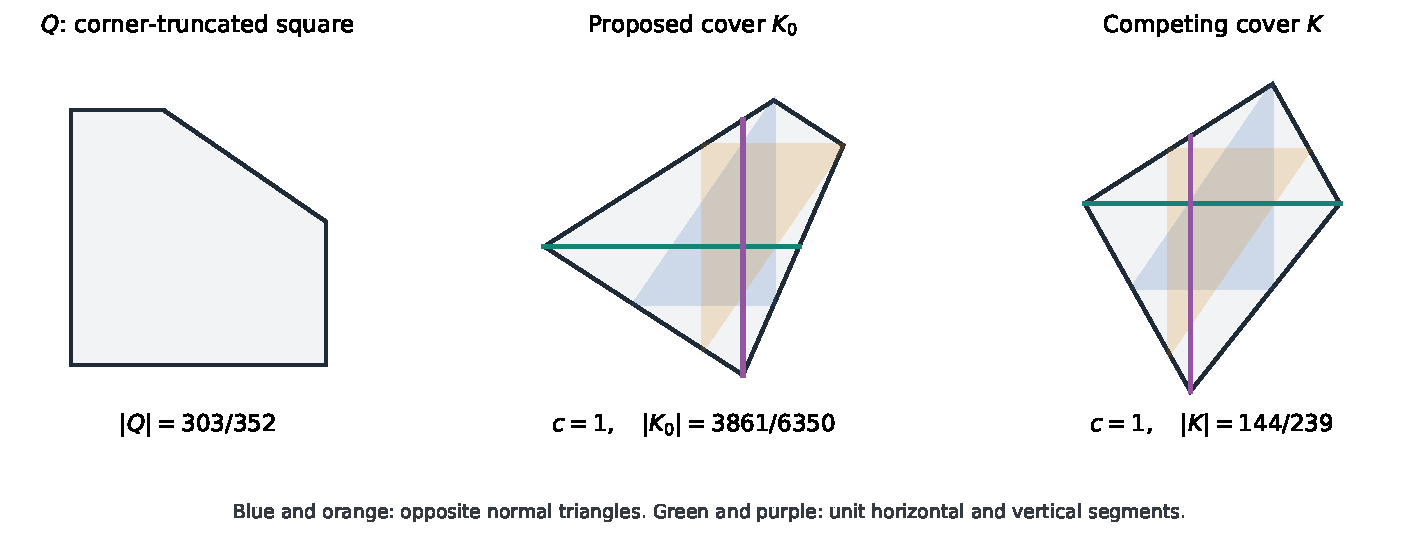
\includegraphics[width=\linewidth]{figures/truncated-covers.pdf}
 \caption{The corner-truncated square, the proposed partner, and the
 competing partner at the exact parameters $A=11/20$, $B=4/5$. The two
 cover panels use the same scale; each contains translations of the four
 unit normal templates.}
 \label{fig:truncated-covers}
\end{figure}

% Optional follow-on to truncated-square-section.tex; same notation and labels.
\subsection{An affine-area deformation through pentagonal covers}

The comparison above comes from a deformation of the proposed cover itself.
It is not merely a comparison between unrelated polygons. Write
$e=AB-g^2>0$ and put
\[
 z_F=\frac{A^2a}{d},\qquad z_M=\frac{A^2a}{e}.
\]
For $z_F\leq z\leq z_M$, define
\[
 D_z=\left(z,\frac gA z-A\right),\quad
 L_z=-\frac aA D_z,\quad R_z=L_z+(1,0),\quad
 t_z=C+\frac gA D_z,
\]
and let
\[
 P_z=\operatorname{conv}\{L_z,D_z,R_z,t_z,C\},\qquad C=(A,B).
\]
At the left endpoint $R_z,t_z,C$ are collinear and $P_{z_F}=K_{A,B}$.
At the right endpoint $D_z,R_z,t_z$ are collinear and $P_{z_M}$ is the
proposed trapezoid $K_0$ of \cite[Figure~11]{BMP2026}.
Indeed its ten template vertices obey exactly the three four-point
collinearities used there to specify $K_0$: the line $L_zD_z$ contains
$0$ and $t_z-C$; the line $D_zt_z$ contains $(A,0)$ and $R_z$;
and the line $L_zC$ contains $t_z-(A,0)$ and $D_z+e_2$.

\begin{proposition}\label{prop:truncated-shadow}
For every $z\in[z_F,z_M]$,
\begin{equation}\label{eq:shadow-cover-area}
 c_{\mathrm{EHZ}}(P_z\times_L Q_{A,B})=1,\qquad
 |P_z|=\frac{1+Ag}{2}+\frac{g(g-A^2)}{2A^2}z.
\end{equation}
For $z_F<z<z_M$, the five displayed vertices are genuine vertices of
$P_z$. All moving templates undergo translations parallel to the same
vector $(1,g/A)$.
\end{proposition}

\begin{proof}
The identities
\[
 d-e=gB>0,\qquad e-ag=B(1-B)>0,\qquad e-Aa=g(1-B)>0
\]
show that
\[
 0<z_F<z_M<\min\{A,A^2/g\}.
\]
The cross products of consecutive edge vectors of the displayed cycle
$L_z,D_z,R_z,t_z,C$ are, in that order,
\[
 1-\frac{gz}{A^2},\quad
 a-\frac{ez}{A^2},\quad
 g\left(-a+\frac{dz}{A^2}\right),\quad
 g\left(A+\frac{az}{A}\right),\quad
 A+\frac{az}{A}.
\]
They are nonnegative, with only the stated endpoint degeneracies. The
vertical levels satisfy
$D_{z,y}<L_{z,y}=R_{z,y}<t_{z,y}<C_y$; the two chains from $D_z$ to
$C$ are consequently monotone, and the cycle is the boundary of the
claimed convex polygon.

The four templates have the placements $T$, $-T+t_z$, $H+L_z$, and
$V+D_z$. Their containment follows from the following segment identities:
\begin{align*}
 0&=L_z+a(D_z-L_z),&
 (A,0)&=D_z+A(R_z-D_z),\\
 t_z-C&=L_z+B(D_z-L_z),&
 D_z+e_2&=L_z+\frac{z}{A^2+az}(C-L_z),\\
 t_z-(A,0)&=L_z+\frac{Bz}{A^2+az}(C-L_z).
\end{align*}
Every coefficient lies strictly between zero and one. Thus the covering
theorem gives capacity at least one.

The horizontal chord $L_zR_z$ has length one and is a longest horizontal
chord. Below its height the chord length increases linearly from zero.
Immediately above it, the derivative of the chord length is negative:
putting $v=t_z-R_z$ and $w=C-L_z$, both $v_y,w_y$ are positive and
\[
 \frac{v_x}{v_y}-\frac{w_x}{w_y}
 =\frac{\det(v,w)}{v_yw_y}<0,
 \qquad
 \det(v,w)=-\frac{ag(A^2+az)}{A^2}.
\]
Horizontal chord length is a concave function of height in a convex
planar body. Hence no horizontal segment longer than one fits, which
proves the reverse capacity inequality. Finally, the shoelace formula
for the five displayed vertices gives \eqref{eq:shadow-cover-area}.
\end{proof}

If $g>A^2$, moving from $z_M$ toward $z_F$ strictly decreases area while
preserving capacity. Thus the proposed optimizer is not even a local
minimum of capacity-one cover area in this parameter region. If
$g<A^2$, the opposite endpoint minimizes area within this particular
family. At $g=A^2$, the entire interval consists of equal-area,
capacity-one covers, including genuine pentagons between the two
trapezoidal endpoints. These assertions concern the explicit deformation;
they do not establish global minimality of either endpoint or of the
intermediate pentagons.


\clearpage
\section{Methods, scope, and companion material}

The action-body construction turns affine capacity optimization into a
support-function and Pfaffian problem. It yields the full-affine pentagon
bound and both simplex bounds. In four dimensions the simplex interaction
graph admits a direct proof; in six dimensions the global equality theorem
also depends on an exact cdd/PPL vertex classification. These are class
bounds, while the HKO intersection uses a complete exact capacity computation
at one moderate parameter. The separate first-variation reduction uses
labeled shortest-orbit measures: seven selected cuts give a seventeen-facet
ascent near $H$, while adding two arbitrary characteristic-invariant affine
hinges and retaining the original facet inequalities cannot give positive
first variation. The latter is a scoped first-order
statement, not a local-maximality theorem for all twelve-facet bodies.
Neither calculation determines the unrestricted
four-dimensional optimum or the maximum along the twenty-facet family.

The planar results use geometric rather than action-polytope reductions.
Shadow deformations and confocal paraboloids give a sharp difference-area
constant for squared bodies, but the Chaidez--Tanny capacity transfer does
not establish a sharp four-dimensional constant. Translation covers and
lattice overlaps give a strict inequality for every partner of a truncated
parallelogram, even though its proposed minimum-area partner fails. The
actual minimizing partner and bounds for intersections of three or more
confocal paraboloids remain open here.

\paragraph{Source and data availability.}
This PDF is report revision \texttt{2026-10-29-r6} and is to travel with its
same-revision source-and-evidence companion archive. That archive supplies
the LaTeX source, figure sources, exact inputs and replay programs under
\path{certificates/}, scoped reviews, and an SHA-256 file manifest. The
finite certificate arrays and full enumeration outputs are not printed in
this PDF. The replay commands and software requirements are in the
respective certificate READMEs. A successful replay checks the stated
finite predicates; the geometric implications are the written proofs here.

\clearpage
\appendix
% Standalone section module; requires amsmath, amssymb, amsthm and the
% theorem/proposition/corollary/remark environments. Bibliography: HK2017,HKO2026.
\section{First variation under simultaneous facet splittings}
\label{sec:multicut-variation}

Fixed-facet variations do not describe the birth of several facets at once.
Here the relevant first-order datum is a convex function on each old facet:
it records the maximum depth of the competing cuts. We obtain its exact
capacity response from labeled occupation measures of shortest polygonal
characteristics. The resulting convex-order criterion is a criterion for
\emph{first-order stationarity}. It does not prove a Hausdorff neighborhood
of local maximality for the pentagon counterexample.

Let $K=\{x\in\mathbb R^{2n}:a_i\cdot x\leq1,\ 1\leq i\leq m\}$
be a bounded polytope containing the origin in its interior, with genuine
facets $F_i$. Here $\mathbb{J}$ is characterized by
$\omega_0(u,v)=\langle\mathbb{J}u,v\rangle$, with $\mathbb{J}^2=-I$.
Its matrix is the negative of the skew-form matrix $J$ in
Section~\ref{subsec:affine-action-body}; throughout this appendix put
$\omega=\omega_0$.
For a finite word of facet labels and weights, put
\begin{equation}\label{eq:mc-word}
 Q(\sigma,\beta)=\sum_{r<s}\beta_r\beta_s
 \omega(a_{\sigma_r},a_{\sigma_s}),\qquad
 \sum_r\beta_ra_{\sigma_r}=0,\quad
 \sum_r\beta_r=1,\quad\beta_r\geq0.
\end{equation}
Haim--Kislev's formula~\cite{HK2017} gives
$Q_*:=\max Q=1/(2c_{\mathrm{EHZ}}(K))$ using words without repeated labels.
Repeated words also satisfy $Q\leq Q_*$: their unit-period polar loop has
velocity $2\mathbb{J}a_{\sigma_r}$ for time $\beta_r$, action $2Q$, and dual energy
$\frac14\int h_K(-\mathbb{J}\dot z)^2=1$. Normalizing its action to one in the dual
action principle gives $c_{\mathrm{EHZ}}(K)\leq1/(2Q)$. Translating the loop
to zero mean changes neither quantity. For redundant rows the support values
are at most one, so the same inequality holds.

We impose the \emph{full-rank support condition}: after deleting
zero weights from any finite maximizing word, the augmented constraint
columns span $\mathbb R^{2n+1}$, or equivalently
\[
 \operatorname{rank}\bigl[(a_{\sigma_r},1)\bigr]_r=2n+1.
\]
This concerns the constraint matrix, not the Hessian of the quadratic program.

A maximizing word reconstructs a shortest boundary characteristic, as shown
below. Parametrize it on $[0,1]$ with velocity $2T\mathbb{J} a_{\sigma_r}$ for time
$\beta_r$, where $T=c_{\mathrm{EHZ}}(K)$. Its labeled occupation measure
$\mu_\gamma$ is a probability on the disjoint union
$X=\bigsqcup_iF_i$: time on a segment with label $i$ is assigned to that
copy of $F_i$, including at ridges. Let $\mathcal M$ be the weak closure of
the measures of \emph{all finite maximizing words}, allowing repetitions.
The normalized cone-volume probability is
\begin{equation}\label{eq:mc-nu}
 d\nu|_{F_i}=\frac{dS}{2n\,\operatorname{Vol}_{2n}(K)|a_i|}.
\end{equation}

\begin{theorem}[Simultaneous-splitting derivative]\label{thm:mc-derivative}
Assume the full-rank support condition. For each facet choose a nonempty
finite list $D_{ij}\in\mathbb R^{2n}$ and set
\[
 K_t=\{x:(a_i+tD_{ij})\cdot x\leq1\text{ for every }i,j\},\qquad
 f_i(x)=\max_jD_{ij}\cdot x\quad(x\in F_i).
\]
For this fixed finite list, the right derivative exists and equals
\begin{equation}\label{eq:mc-derivative}
 \left.\frac{d}{dt}\right|_{0+}
 \log\frac{c_{\mathrm{EHZ}}(K_t)^n}{n!\operatorname{Vol}_{2n}(K_t)}
 =2n\left(\int_X f\,d\nu-
                  \max_{\mu\in\mathcal M}\int_X f\,d\mu\right).
\end{equation}
In particular, the hypothesis holds for every Lagrangian product of two
planar polygons having no antipodal facet normals, including the HKO product.
\end{theorem}

\begin{proof}
We give the sensitivity and placement arguments explicitly, since neither
requires a smooth optimizing branch.

\emph{A local chart at every limiting optimizer.}
For the fixed augmented row list, the moving optimum $q(t)$ is the maximum
over finitely many permutations and their feasible weights. This remains
true with redundant or repeated presentation rows: genuine facets give one
inequality and the polar-loop bound above gives the other. Along any sequence
$t\downarrow0$, compactness of the weight simplex and finiteness of the words
give maximizing weights $\beta_t\to\beta_0$ in one word. Capacity continuity
makes $\beta_0$ a base maximizer.
Choose $2n+1$ positive coordinates $I$ forming an invertible constraint minor,
and denote the remaining weights by $z$. With columns
$B_r(t)=(a_{\sigma_r}+tD_r,1)$, solve
\[
 \beta_I(t,z)=B_I(t)^{-1}\bigl(e-B_J(t)z\bigr),
 \qquad e=(0,\ldots,0,1)^T.
\]
The solved weights stay positive near $(0,z_0)$; the other coordinates merely
satisfy $z\geq0$. In particular $\beta(0,z_t)$ is base-feasible.
Writing $F(t,z)=Q_t(\beta(t,z))$, we obtain
\[
 q(t)-Q_*\leq F(t,z_t)-F(0,z_t)
             =t\,\partial_tF(0,z_0)+o(t).
\]
Conversely the section with $z=z_0$ fixed gives the reverse lower bound for
every base optimizer. Thus $q'(0+)$ exists and is the maximum of these
section derivatives. This comparison also covers singular Hessians and
continua of maximizing weights.

\emph{Placement of a maximizing word.}
Delete zero weights and write $a_r=a_{\sigma_r}$,
$s_r=\sum_{k<r}\beta_ka_k$, and $p_r=\partial_{\beta_r}Q$.
Stationarity and full rank give unique multipliers satisfying
\[
 p_r=\lambda\cdot a_r+\eta,
 \qquad \eta=2Q_*=1/T,
 \qquad p_r=-2\omega(a_r,s_r)=2a_r\cdot \mathbb{J}s_r.
\]
The vertices $x_r=-T\lambda+2T\mathbb{J}s_r$ therefore satisfy $a_r\cdot x_r=1$.
The segment to $x_{r+1}$ has direction $\mathbb{J}a_r$, so its active facet equation
holds throughout. To obtain every other facet inequality, insert an arbitrary
normal $a_k$ at any point of the loop, subdividing its current segment if
necessary. Give the inserted row weight $\varepsilon\geq0$ and compensate
with the positive minor. Its reduced objective derivative is
\[
 p_{\rm new}-\lambda\cdot a_k-\eta
   =\frac{a_k\cdot x-1}{T}.
\]
Global optimality among repeated words makes this nonpositive. Hence the
whole loop lies in $K$, on its labeled facets, and has action $T$.

\emph{The midpoint formula.}
Differentiate a feasible section of this word with row velocities $D_r$.
The differentiated constraints give
$\sum_ra_r\beta'_r=-\sum_r\beta_rD_r$ and $\sum_r\beta'_r=0$.
The direct row derivative of $Q$ is
\[
 \sum_r\bigl[-2\beta_r\omega(D_r,s_r)
              -\beta_r^2\omega(D_r,a_r)\bigr].
\]
Adding the weight derivative $-\sum_r\beta_r\lambda\cdot D_r$ yields
\begin{equation}\label{eq:mc-midpoint}
 \begin{aligned}
 Q'&=\frac1T\sum_r\beta_rD_r\cdot x_r^{\rm mid},\\
 x_r^{\rm mid}&=x_r+T\beta_r\mathbb{J}a_r.
 \end{aligned}
\end{equation}
The self term in the preceding display is essential: the evaluation point
is the segment midpoint, not its starting point.
For every optimizer in the finite bank, $D_r\cdot x\leq f_i(x)$ on its
segment labeled $i$. Affine midpoint integration therefore gives
$q'(0+)\leq T^{-1}\max_{\mathcal M}\int f\,d\mu$.
For the reverse inequality, take any finite maximizing base word and
subdivide every segment at the finitely many switches of the maximum
$f_i=\max_jD_{ij}\cdot x$. Assign a maximizing row on each resulting interval.
After deleting zero-length pieces, this is a positive repeated word with the
same base objective and full rank. A feasible continuation exists, and the
polar-loop inequality bounds its objective by $q(t)$.
Equation~\eqref{eq:mc-midpoint} now integrates $f$ exactly. Taking the supremum
and then weak closure gives
\[
 q'(0+)=2Q_*\max_{\mu\in\mathcal M}\int f\,d\mu,
 \qquad \frac{c'(0+)}{c(K)}=-2\max_{\mu\in\mathcal M}\int f\,d\mu.
\]
The maximum over $\mathcal M$ exists because $X$ is compact.

\emph{Volume and the product hypothesis.}
Away from the ridges, the radial gauge of $K_t$ has derivative $f_i$ on
$F_i$. The radial volume formula and dominated convergence, using the fixed
finite row list, give
\[
 V'(0+)=-\sum_i\int_{F_i}\frac{f_i}{|a_i|}\,dS
        =-2nV\int f\,d\nu.
\]
This proves~\eqref{eq:mc-derivative}.
For a planar Lagrangian product, a positive-$Q$ word must use both factors.
Closure separates into the two planes. A positive closed combination of
nonzero planar normals without antipodal pairs spans its plane; hence the
active normals span $\mathbb R^4$. If $v\cdot a_r+s=0$ on their positive
support, weighting and summing gives $s=0$, then $v=0$. The augmented rank is
therefore five, also for repeated words.
\end{proof}

\begin{corollary}[A common convex-order ensemble]\label{cor:mc-convex-order}
Under the theorem's hypothesis, the following are equivalent:
\begin{enumerate}[label=\textup{(\roman*)}]
\item Every fixed finite simultaneous-splitting direction has nonpositive
first systolic variation.
\item The weakly closed convex hull of $\mathcal M$ contains a probability
$\bar\mu$ such that
$\int f\,d\bar\mu\geq\int f\,d\nu$ for every continuous function convex
on each facet copy.
\end{enumerate}
It is enough in \textup{(i)} to use inward cuts retaining every old facet.
Any such $\bar\mu$ has the same mass and first moment as $\nu$ on each facet.
\end{corollary}
\begin{proof}
Finite maxima of affine functions are uniformly dense in the continuous
convex functions on a compact facet. Every affine function there is $D\cdot x$
because $a_i\cdot x=1$. Thus the theorem turns (i) into
$\sup_{\mathcal M}\int f\,d(\mu-\nu)\geq0$ for every facetwise convex $f$.
Let $B=\overline{\operatorname{conv}}\mathcal M$. For a finite list
$f_1,\ldots,f_k$, the compact convex set of vectors
$(\int f_j\,d(\mu-\nu))_{j=1}^k$, $\mu\in B$, meets the positive orthant.
Otherwise separation supplies nonnegative coefficients $\alpha_j$ whose
sum $\sum_j\alpha_jf_j$ contradicts the preceding inequality.
Compactness and the finite-intersection property now give one common
$\bar\mu$ for all $f$. The converse is immediate.
Adding one common large constant to all facet profiles makes them
nonnegative, allowing the zero row to be retained; the difference of two
probability integrals annihilates that constant. Finally test both signs of
facetwise affine functions to obtain the mass and first-moment identities.
\end{proof}

The common-ensemble requirement is stronger than finding a different
successful orbit for each single cut. Nor does first-order nonincrease give
an unrestricted neighborhood theorem: zero derivatives and estimates whose
constants deteriorate with cut count or slope still require analysis.

\subsection{Two limitations of finite orbit reductions}

The HKO body is $H=P\times_LR(-\pi/2)P$, where $P$ is the circumradius-one
regular pentagon. Put $\alpha=\pi/5$, $\tau=\tan\alpha$, and
\[
 a_0=(1,\tau,0,0),\qquad w=(-\sin\alpha,\cos\alpha).
\]
On $F_0=E_0\times R(-\pi/2)P$, the functional $\ell(q,p)=w\cdot p$
attains its maximum one exactly on $E_0\times\{w\}$.

\begin{proposition}[No finite pure-word ensemble is universal]
No finite convex combination of occupation measures of finite pure
facet-word characteristics of $H$ dominates $\nu$ for every facetwise convex
profile. Here a pure segment has velocity a positive multiple of one
$\mathbb{J}a_i$ and carries that label; shortestness is not required.
\end{proposition}
\begin{proof}
On a segment labeled zero, $\ell$ is constant since
$w\cdot(1,\tau)=0$. Its value is strictly below one: a nonconstant
p-segment cannot lie in the singleton exposing slice at $w$.
A finite bank therefore has a common bound $\ell\leq h<1$ on all its
zero-labeled segments. For $h<r<1$, the profile
$f_0=(\ell-r)_+$, $f_i=0$ for $i\ne0$, vanishes on the bank but has
positive $\nu$-integral. It is realized by the single extra row
$a_0+t(-r,-r\tau,w_1,w_2)$.
More explicitly, for $\delta=1-r<1-\cos(2\alpha)$, the pentagon cap
has slice width $2z\cot\alpha$, so
\[
 \int_Xf\,d\nu=\frac{\cot\alpha}{30\operatorname{area}(P)}\delta^3>0.
\]
\end{proof}

A separate computer-assisted theorem, sourced in
Section~\ref{sec:hko-ascent}, establishes that $H$ is a Hausdorff local
maximizer of $\rho$ among convex four-polytopes with at most eleven
genuine facets.
The proposition shows why no fixed finite bank of pure facet-word measures
can dominate all convex profiles. It is compatible with that eleven-facet
theorem and with the twenty-facet ascent of Section~\ref{sec:hko-ascent}.
Infinite ensembles and weak limits remain available in
Corollary~\ref{cor:mc-convex-order}.
For an action-$T$ word, the wedge at $w$ also gives the quantitative bound
$1-\ell\geq T\beta\sec\alpha\tan\alpha$ on a zero-labeled segment of
weight $\beta$, by comparing its length with the wedge's slice width.

A second obstruction concerns eliminating repeated normals by moving their
weights to an endpoint. That operation need not maximize a convex profile's
occupation response, even along a family of genuine HKO minimizers.
For the following explicit example set $r=\sqrt5$, $\tau=\sqrt{5-2r}$,
$u=(3-r)/2$, $v=\tau(1+r)/2$, and $s=r-1$. The ten normals are
\[
\begin{split}
 &(1,\tau,0,0),\ (-u,v,0,0),\ (-s,0,0,0),\ (-u,-v,0,0),\ (1,-\tau,0,0),\\
 &(0,0,\tau,-1),\ (0,0,v,u),\ (0,0,0,s),\ (0,0,-v,u),\ (0,0,-\tau,-1).
\end{split}
\]

\begin{proposition}[An interior response maximum]\label{prop:mc-interior}
Let $b=(5-r)/20$ and consider
\[
 \sigma=(0,6,7,3,2,8,3,9),\qquad 0\leq q\leq1,
\]\[
 \beta(q)=\left(\frac r{10},\frac{5+r}{40},\frac{5-r}{40},
 b(1-q),b,\frac{5-r}{40},bq,\frac{5+r}{40}\right).
\]
Every member is a maximizing word. For the facetwise convex profile
$f_3(x)=|x-c_3|^2$, $f_i=0$ otherwise, where
$c_3=(-1/4,\tau(\tau^2-9)/8,0,0)$ is the facet centroid, its response is
\[
 g(q)=\int f\,d\mu_q
 =\frac{2-r}{4}q^2+\frac{-19+9r}{16}q+\frac{195-77r}{240}.
\]
Its maximum occurs at $q_*=(7-r)/8$ and satisfies
$g(q_*)-\max\{g(0),g(1)\}=(r-1)/128>0$.
\end{proposition}
\begin{proof}
Substitution gives closure and $Q=\tau/5$ at both endpoints. The objective
is affine in the transfer between two identical normals, since
$\omega(a_3,a_3)=0$, so it is constant throughout. This is the HKO optimum
by~\cite{HKO2026}; the placement argument above applies.
For a direct calculation of the response, the two row-three segment
midpoints are
\[
 \begin{aligned}
 m_1(q)&=\frac14\bigl(-1-r,-\tau(1+r),\tau(r+q),1+rq\bigr),\\
 m_2(q)&=\frac14\bigl(-1,-\tau(2+r),\tau(q-3-r),1-r+rq\bigr).
 \end{aligned}
\]
Their weights are $b(1-q)$ and $bq$. Exact integration of a quadratic along
a straight segment of weight $\beta$ gives
$\beta(|m-c_3|^2+T^2\beta^2|a_3|^2/3)$.
Here $T=5/(2\tau)$ and $T^2b^2|a_3|^2/3=(5-r)/24$.
Inserting the displayed midpoints yields $g$; differentiating this
strictly concave quadratic proves the claimed maximum and gap.
\end{proof}

Uniform approximation of this profile by finite maxima of affine functions
preserves the strict endpoint gap. Thus the phenomenon also occurs for a
finite inward split bank. It refutes the proposed convexity argument for
deleting repetitions; it does not show that the two displayed endpoint words
are best among \emph{all} simple HKO words, and does not exhibit an improving
systolic variation.

\section{A quantitative near-zero remainder for the HKO cuts}
\label{sec:hko-effective}

The derivative argument can be made effective without enumerating all
twenty-row permutations. Its numerical step is deliberately tiny and
illustrates quantitative control of the true capacity. The separate exact
computation in Theorem~\ref{thm:hko-finite-improvement} gives a substantially
larger ratio increase at a moderate parameter.

\begin{proposition}[Effective improvement]\label{prop:hko-effective}
For the original family~\eqref{eq:ha-family}, with all ten unit-speed cuts,
\[
 \frac{\operatorname{sys}(H_t)}{\operatorname{sys}(H)}
       >1+\frac{t}{200},\qquad 0<t\leq10^{-30}.
\]
\end{proposition}

We give the analytic estimates, including the uniform pivot and the passage
from near-maximizers to exact base maximizers. The finite primitive action
gap and rational constant comparisons have an exact replay; see
\path{certificates/hko-ascent/README.md}.

Put $q(t)=1/(2c_{\EHZ}(H_t))$, $q_0=\tau/5$, and
$V_0=\Vol_4(H)$. The twenty presentation rows have the form
$a_r+tD_r$: one copy of each base normal has $D_r=0$, and its other copy
has the velocity in~\eqref{eq:ha-directions}. A simple word in this bank
therefore contains at most two occurrences of each base normal. For an
ordered word, let
\[
 B_r(t)=(a_r+tD_r,1),\qquad e=(0,0,0,0,1)^{\mathsf T},
 \qquad Q_t(\beta)=\tfrac12\beta^{\mathsf T}G_t\beta,
\]
where $G_t$ is the symmetric ordered-action matrix. Write $D$ for the
matrix whose columns are $(D_r,0)$. Feasibility means
$B(t)\beta=e$ and $\beta\geq0$. The Haim--Kislev formula supplies a
maximizing simple word for every $t$, while $H_t\subset H$ gives
$q(t)\geq q_0$. The all-word response bound proved in
Lemma~\ref{lem:ha-repeat} and Proposition~\ref{prop:ha-certificate} implies
that every exactly maximizing base word with a feasible smooth
continuation has action derivative at most
\begin{equation}\label{eq:he-base-derivative}
 g_*=\frac{2q_0}{125}.
\end{equation}
Indeed, the midpoint identity~\eqref{eq:mc-midpoint} makes that derivative
$2q_0\sum_r\beta_rD_r\cdot x_r^{\rm mid}$, bounded by $2q_0$ times the
total radial-hinge response. Repeated occurrences are covered by the
proved reduction, not by an assumption that all maximizers are simple.
The exact primitive calculation also gives
\begin{equation}\label{eq:he-primitive-gap}
 \Delta=\frac{-\tau+3\tau^3}{20}>\frac1{50}
\end{equation}
as the minimum positive loss from $q_0$ among the $3000$ triangle-pair
cyclic six-orders. These finite predicates are checked in the companion;
the following implications are analytic.

\begin{lemma}[A positive pivot for moving near-maximizers]
\label{lem:he-pivot}
Let $0\leq t\leq10^{-3}$, and let a feasible nonnegative simple word on the
twenty-row bank have $Q_t(\beta)\geq q_0/2$. Five positive coordinates
$I$ have weights greater than $1/4500$, and their augmented base columns
form an invertible matrix $B_I(0)$ satisfying
\[
 |\det B_I(0)|>\tfrac12,\qquad
 \|B_I(0)^{-1}\|_2<66,\qquad
 \|B_I(0)^{-1}\|_\infty<200.
\]
\end{lemma}

\begin{proof}
Let $N=\sqrt5-1=|a_r|$. Both retained and moved rows obey
$|D_r|\leq\sqrt{1+(3N/5)^2}<5/4$, while $N<5/4$.
Bilinearity and $\sum_{r<s}\beta_r\beta_s\leq1/2$ give
\[
 |Q_t(\beta)-Q_0(\beta)|
 \leq\frac{25}{16}t+\frac{25}{32}t^2
 <\frac1{60}<\frac{q_0}{6}.
\]
Here $Q_0(\beta)$ uses the base normals but need not have base closure.
Thus $Q_0(\beta)>q_0/3>1/30$. If $s$ is the total $q$-factor mass,
write $Q_0=s(1-s)B(x,y)$ for normalized occurrence distributions in
the two factors. Each cross pairing has absolute value at most
$N^2<25/16$, so $|B(x,y)|\leq25/16$ and
\[
 s,1-s\geq s(1-s)>\frac8{375}.
\]

Perturbed closure gives the base residual directly, including the
retained rows with zero velocity:
\[
 \left\|\sum_r\beta_ra_r\right\|
 =t\left\|\sum_r\beta_rD_r\right\|
\leq\tfrac54t\leq2t.
\]
After division by either factor mass, the mean residual of its
normalized pentagon-direction distribution is at most
$2t/(8/375)\leq3/32<1/8$. Passing from normals of length $N>1$
to unit normals only decreases it.

Aggregate each normalized factor distribution by its five normal
directions and order those masses decreasingly. Let $r$ be the sum of
the three smallest. The resultant of the two largest unit directions
has norm at least $(1-r)\cos72^\circ>(1-r)/4$; the other three
contribute at most $r$ in the opposite direction. A mean norm below
$1/8$ therefore forces $r>1/16$. Each of the three largest masses is
at least $r/3>1/48$. Multiplying by the factor mass gives aggregate
weight greater than $1/2250$ on each chosen direction. At most two row
occurrences represent one direction, so one occurrence has weight
greater than $1/4500$.

Choose two distinct $q$ directions and three distinct $p$ directions
among these. Their five augmented columns are independent. The
absolute determinant is the product of a two-normal planar determinant
$N^2|\sin(k\pi/5)|>1/2$ and a three-normal affine determinant, which
has one of the exact values $(5\tau+\tau^3)/2$ or $5\tau-\tau^3$,
both greater than one. Thus the five-column determinant exceeds
$1/2$. Each augmented column has norm
$\sqrt{1+N^2}=\sqrt{7-2\sqrt5}<8/5$. Hadamard's inequality bounds
each cofactor by $(8/5)^4<6.56$ and the adjugate's Frobenius norm by
$32.8$. Dividing by the determinant yields
$\|B_I(0)^{-1}\|_2<66$ and hence
$\|B_I(0)^{-1}\|_\infty<200$.
The argument is independent of word order and includes zero-velocity
old rows. For completeness, perturbing these five columns by
$tD_I$ changes their determinant by at most
$5(5/4)t(1.61)^4<1/8$ on the stated interval; the moving minor also
stays invertible.
\end{proof}

\begin{proof}[Proof of Proposition~\ref{prop:hko-effective}]
Fix $0<t\leq10^{-30}$ and a simple word attaining $q(t)$, with weights
$\beta_t$. It satisfies the lemma because $q(t)\geq q_0$.
Set $M=200$, and keep the nonpivot weights $z=(\beta_t)_J$ fixed.
Solve the five pivot weights for $0\leq s\leq t$ by
\begin{equation}\label{eq:he-chart}
 \beta_I(s)=B_I(s)^{-1}\bigl(e-B_J(s)z\bigr),\qquad
 \beta_J(s)=z.
\end{equation}
Let $\beta_0=\beta(0)$. Since $B(0)\beta_t=e-tD\beta_t$,
\[
 \beta_{0,I}-(\beta_t)_I
       =tB_I(0)^{-1}D\beta_t.
\]
The last row of $D$ is zero. Using $|D_r|<2$ gives an infinity-norm
change at most $2Mt$. Hence every pivot of $\beta_0$ exceeds
$1/4500-400\cdot10^{-30}>c:=10^{-4}$. The other weights are unchanged;
$\beta_0$ is a base-feasible probability vector on the same word.

Here are uniform chart bounds, valid more generally for
$0\leq s\leq10^{-8}$. The infinity norm of the five-column
perturbation matrix is at most ten. The Neumann bound gives
$\|B_I(s)^{-1}\|_\infty\leq2M$. The exact difference and differentiated
constraint equations are
\[
 \begin{aligned}
 \beta_I(s)-\beta_{0,I}&=-sB_I(s)^{-1}D\beta_0,\\
 \beta'_I(s)&=-B_I(s)^{-1}D\beta(s),\\
 \beta''_I(s)&=-2B_I(s)^{-1}D_I\beta'_I(s).
 \end{aligned}
\]
Thus $\|\beta(s)\|_1\leq1+20Ms<2$,
$\|\beta'(s)\|_1\leq40M$, and
$\|\beta''(s)\|_1\leq1600M^2$. For the last bound, each
coordinate of $\beta'_I$ has magnitude at most $8M$, each
coordinate of $\beta''_I$ at most $320M^2$, and there are five.
These estimates concern the algebraic chart; its weights need not
stay positive throughout the larger auxiliary interval.

Put $F(s)=Q_s(\beta(s))$. Each moving normal has norm below two there,
so entries of $G_s,G'_s,G''_s$ are bounded in absolute value by
$4,8,8$, respectively. Differentiation gives
\[
\begin{aligned}
 |F''(s)|
 &\leq4\bigl[(40M)^2+2(1600M^2)\bigr]\\
 &\quad+2\cdot8\cdot(40M)\cdot2+\tfrac12\cdot8\cdot2^2\\
 &=19200M^2+1280M+16<2\cdot10^5M^2.
\end{aligned}
\]
With $R=10^5M^2=4\cdot10^9$, Taylor's theorem yields
\begin{equation}\label{eq:he-taylor}
 q(t)=F(t)\leq Q_0(\beta_0)+t\,g(\beta_0)+Rt^2,
\end{equation}
where $g$ is the derivative at zero of the fixed-pivot algebraic
chart. For any base-feasible probability vector $\beta$ on this word,
\[
 g(\beta)=\tfrac12\beta^{\mathsf T}G'_0\beta
                 +(G_0\beta)\cdot u(\beta),\qquad
 u_I(\beta)=-B_I(0)^{-1}D\beta,\quad u_J=0.
\]
The bounds $\|u(\beta)\|_1\leq10M$,
$\max|G_0|\leq4$, and $\max|G'_0|\leq8$ imply
\begin{equation}\label{eq:he-lipschitz}
 |g(\beta)|\leq4+40M\leq44M,\qquad
 |g(\beta)-g(\beta')|\leq88M\|\beta-\beta'\|_1
\end{equation}
for base-feasible probability vectors $\beta,\beta'$ on this word.
The direct quadratic term contributes at most $8\|\beta-\beta'\|_1$;
the other term contributes at most $80M\|\beta-\beta'\|_1$.

Let $d=q_0-Q_0(\beta_0)\geq0$. From $q(t)\geq q_0$,
\eqref{eq:he-taylor}, and~\eqref{eq:he-lipschitz},
\begin{equation}\label{eq:he-small-deficit}
 d\leq44Mt+Rt^2<10^{-20},
 \qquad Q_0(\beta_0)>q_0/2.
\end{equation}
We now round $\beta_0$ to an exact maximizing base word without
changing its order or losing the positive pivot.

Let $s$ be its $q$-factor mass and let $u,v$ be its normalized
factor weights. Each occurrence-wise planar closure polytope has at
most forty vertices: each vertex uses one of five closing triangles
and one of at most two occurrences of each of its three normals.
The same count holds for a subword, which defines a face of the
full occurrence polytope. Write convex decompositions
$u=\sum_i\lambda_i u_i$ and $v=\sum_j\gamma_jv_j$, with at most forty
vertices per factor. If $q_{ij}$ is the action of triangle pair
$(u_i,v_j)$ at balanced factor mass in this fixed order, put
$S=\sum_{ij}\lambda_i\gamma_jq_{ij}$. Then
\begin{equation}\label{eq:he-deficit}
 Q_0(\beta_0)=4s(1-s)S,\qquad
 d=4q_0(s-\tfrac12)^2+4s(1-s)(q_0-S).
\end{equation}
Every $q_{ij}\leq q_0$, and every strict loss is at least
$\Delta$ from~\eqref{eq:he-primitive-gap}. As
$Q_0(\beta_0)>q_0/2$, we have $4s(1-s)>1/2$.
If $\varepsilon$ is the total product mass of nonwinning pairs,
\begin{equation}\label{eq:he-bad-mass}
 \varepsilon\leq\frac{q_0-S}{\Delta}\leq\frac{2d}{\Delta},
 \qquad 2|s-\tfrac12|\leq\sqrt{d/q_0}.
\end{equation}

For $\varepsilon>0$, delete from each marginal every vertex whose
coefficient is less than $2\sqrt\varepsilon$ and renormalize.
At most forty vertices are deleted per marginal, so the discarded
mass is at most $80\sqrt\varepsilon<1$ by
\eqref{eq:he-small-deficit}. A surviving bad pair would have product
mass at least $4\varepsilon$, contradicting the definition of
$\varepsilon$. Thus all surviving pairs win. If $\varepsilon=0$,
keep the original positive supports. Denote the resulting mixtures
by $u^*,v^*$ and put $\beta^*=(u^*/2,v^*/2)$ on the same ordered
occurrences. It is base-feasible and $Q_0(\beta^*)=q_0$.
Each marginal changes by at most $160\sqrt\varepsilon$ in
$\ell^1$, so~\eqref{eq:he-bad-mass} gives
\begin{equation}\label{eq:he-rounding}
 \|\beta_0-\beta^*\|_1
 \leq 2|s-\tfrac12|
       +\tfrac12\|u-u^*\|_1+\tfrac12\|v-v^*\|_1
 \leq\left(\frac1{\sqrt{q_0}}
             +160\sqrt{\frac2\Delta}\right)\sqrt d
 \leq2000\sqrt d.
\end{equation}
By~\eqref{eq:he-small-deficit}, this is less than
$2\cdot10^{-7}<c/2$. Every selected pivot weight of $\beta^*$
is therefore positive. The same fixed-pivot chart gives a feasible
smooth continuation through this exact base maximizer.
Its derivative obeys~\eqref{eq:he-base-derivative}, and
\eqref{eq:he-lipschitz}--\eqref{eq:he-rounding} give
\[
 g(\beta_0)\leq g_*+A\sqrt d,\qquad
 A=88M\cdot2000=35\,200\,000.
\]
This applies the response bound only to an exact maximizing word;
the near-maximizer is handled by the quantified rounding.

Substituting into~\eqref{eq:he-taylor} and maximizing
$-d+At\sqrt d$ over $d\geq0$ by completing the square gives a
bound for the \emph{true global} action:
\begin{equation}\label{eq:he-global-action}
 q(t)\leq q_0+g_*t+(A^2/4+R)t^2
       \leq q_0+\frac{2q_0}{125}t+10^{15}t^2.
\end{equation}
Indeed $A^2/4+R=309\,764\,000\,000\,000<10^{15}$.
No selected feasible branch is substituted for the global optimum.

For volume, on an old facet the gauge of $H_t$ is at least
$1+tf_i$, because the old and moved rows both occur. Other
inequalities only increase the gauge. The normalized cone-volume
measure $\nu$ of~\eqref{eq:mc-nu} and the radial volume formula yield
\[
 \frac{\Vol_4(H_t)}{V_0}
 \leq\int(1+tf)^{-4}\,d\nu
 \leq1-4\nu[f]t+\frac85t^2.
\]
Here $0\leq f_i\leq2/5$, and the second derivative of
$(1+u)^{-4}$ is at most twenty for $u\geq0$.
Put $a=2/125$, $v=4\nu[f]$, and use~\eqref{eq:ha-volume}:
\[
 \eta:=v-2a=\frac{20+64\sqrt5}{9375}>\frac1{100}.
\]
As $q_0>1/10$, \eqref{eq:he-global-action} gives
\[
 \left(\frac{q(t)}{q_0}\right)^2
 \leq(1+at+10^{16}t^2)^2
 \leq1+2at+3\cdot10^{16}t^2.
\]
Multiplying this nonnegative bound by the volume bound and
discarding only negative cross terms gives
\[
 \frac{q(t)^2\Vol_4(H_t)}{q_0^2V_0}
 \leq1-\eta t+4\cdot10^{16}t^2
 <1-\frac{t}{200},
\]
because $4\cdot10^{16}t<1/200$ on the stated interval.
Finally $\operatorname{sys}(H_t)=1/(8q(t)^2\Vol_4(H_t))$,
so taking reciprocals proves the proposition.
\end{proof}

At $t=10^{-30}$ this gives only the certified lower bound
$5\cdot10^{-33}$ on relative gain. The reusable ingredient is the
uniform quadratic remainder for the global optimal action; determining
the maximum along the family remains a separate problem.

\section{Two characteristic-invariant cuts on the HKO product}
\label{sec:ha-two-hinge-proof}

We prove Proposition~\ref{prop:ha-two-hinge}. All old HKO inequalities
remain in the moving bank. The exact family predicates and replay
instructions are at \path{certificates/hko-two-hinge/README.md}.

\paragraph{Quotient coordinates and volume.}
The facet-transitive symmetries used in Proposition~\ref{prop:ha-weighted}
reduce the proof to the q-facet labeled zero. Put
\[
 r=\sqrt5,\quad N=r-1,\quad e=J_2n_0/N,\quad
 m=\frac{1-\cos(\pi/5)}2,\quad h=\frac{1+\cos(\pi/5)}2,
\]
and on that facet use
\[
 \xi=\frac{e\cdot q}{\sin(\pi/5)},\qquad
 \eta=\frac{e\cdot p-m}{h}.
\]
The quotient ranges over $[-1,1]^2$. Every affine function invariant along
$\mathbb{J}a_0$ is $\alpha\xi+\beta\eta+\gamma$: its normal coordinate is constant
on the facet, and invariance excludes precisely the remaining partner
coordinate. Under facet-uniform measure, $\xi$ is uniform on $[-1,1]$ and
independent of $\eta$. Put
\[
 k=r-2,\qquad a=\frac{5-r}{20},\quad b=\frac r{10},\qquad
 A=\frac a2,\quad B=\frac{5+r}{40},\quad C=\frac{5+2r}{10}.
\]
Projection of the partner pentagon gives the probability density
\begin{equation}\label{eq:ha-quotient-density}
 p(y)=\begin{cases}b(y+3),&-1\leq y\leq k,\\
                   C(1-y),&k\leq y\leq1,
       \end{cases}
 \qquad \mu:=\int yp(y)\,dy=-1+\frac{2r}{5}.
\end{equation}
Indeed its vertex projection levels are $-1,k,1$, and the transverse slice
width is affine between them. The exact projection, normalization and mean
are also checked in the accompanying four-family certificate. Each facet
has cone-volume mass $1/10$, so
\begin{equation}\label{eq:ha-quotient-volume}
 \nu(f_0)=\frac1{10}\mathbb E
                (\alpha\xi+\beta\eta+\gamma)_+.
\end{equation}

\paragraph{Four literal shortest-word families.}
The following families realize each edge coordinate $\xi=\pm1$ and every
listed value of $\eta=y$. The facet-zero occupation weight is
\begin{equation}\label{eq:ha-two-weight-curves}
 \beta_L(y)=A(y+3)\quad(-1\leq y\leq k),\qquad
 \beta_U(y)=B(1-y)\quad(k\leq y\leq1).
\end{equation}
At the common endpoint, $\beta_L(k)=b$ whereas $\beta_U(k)=a$; the two
families need not join with the same weight.
Here are their complete ordered words and parameter intervals:
\[
\begin{array}{c|c|c|l}
 \text{family}&\xi& y(z),\quad0\leq z\leq1&\sigma\\ \hline
 L_+& 1&-1+(k+1)z&(0,1,7,6,3,2,9)\\
 L_-&-1&-1+(k+1)z&(0,6,3,2,9,8,4)\\
 U_+& 1& k+(1-k)z&(0,7,3,9,4,5,1)\\
 U_-&-1& k+(1-k)z&(0,4,6,5,2,1,8)
\end{array}
\]
In each listed order, the full weight vector is
$\beta(z)=(1-z)\beta^-+z\beta^+$, with
\[
\begin{array}{c|c|c}
 &\beta^-&\beta^+\\ \hline
 L_+&(a,a,a,a,b,0,b)&(b,0,a,a,a,a,b)\\
 L_-&(a,b,0,b,a,a,a)&(b,b,a,a,a,a,0)\\
 U_+&(a,b,b,a,0,a,a)&(0,b,a,a,a,a,b)\\
 U_-&(a,a,a,a,b,0,b)&(0,b,a,a,a,a,b)
\end{array}
\]
These are catalogue charts 115, 148, 72 and 19, with their parameters oriented
to make $y$ increase. Direct exact arithmetic checks closure, nonnegative
weights and $Q=\tau/5$ at both endpoints and the midpoint. The KKT
reconstruction checks all facet inequalities at all loop vertices,
$\xi=\pm1$, the displayed affine $y$ coordinate, and
\eqref{eq:ha-two-weight-curves}. Endpoint checks extend to the whole family:
the weights and reconstructed positions are affine, and the objective is
quadratic. Interior weights are positive. Only the existence of these four
shortest families is needed below; no numerical search result is a premise.

\begin{lemma}[Scalar hinge bound]\label{lem:ha-scalar-amplification}
For $g(y)=(uy+v)_+$, set
\[
 I(g)=\int_{-1}^1g(y)p(y)\,dy,\qquad
 M(g)=\max\left\{\sup_{[-1,k]}A(y+3)g(y),\
                       \sup_{[k,1]}B(1-y)g(y)\right\}.
\]
Then $I(g)\leq5M(g)$.
\end{lemma}

\begin{proof}
Constants follow from $M(g)\geq bg$ and $5b=r/2>1$.
Positive homogeneity reduces the other cases to decreasing hinges
$(z-y)_+$ and increasing hinges $(y-z)_+$, for real thresholds $z$.

For a decreasing hinge with $z\leq-1$ the claim is trivial. On $[-1,1]$,
convexity in $z$ bounds its integral by the endpoint secant:
\[
 I(z)\leq\frac{z+1}{2}(1-\mu),\qquad M(z)\geq2A(z+1).
\]
The required comparison follows from
$20A-(1-\mu)=(5-r)/10>0$.
For $z\geq1$ the hinge is affine on the support and $I(z)=z-\mu$.
Put $z_0=2k+3=2r-1$ and $z_*=1+4r/5$. When $1\leq z\leq z_0$,
the lower-family point $y=(z-3)/2$ gives $M(z)\geq A(z+3)^2/4$ and
\begin{equation}\label{eq:ha-scalar-square}
 \frac{5A}{4}(z+3)^2-(z-\mu)
       =\frac{5A}{4}(z-z_*)^2\geq0.
\end{equation}
For $z\geq z_0$, use $y=k$ and $M(z)\geq b(z-k)$.
The difference $5b(z-k)-(z-\mu)$ is increasing, since $5b-1>0$,
and is nonnegative at $z_0$ by~\eqref{eq:ha-scalar-square}.

For an increasing hinge with $z\geq1$ the claim is trivial. If $z\leq-1$,
then $I(z)=\mu-z$ and $M(z)\geq b(k-z)$. The difference of these bounds
is smallest at $z=-1$, where
$5b(k+1)-(\mu+1)=(25-9r)/10>0$.
For $-1\leq z\leq k$, integration of the lower density gives
\begin{equation}\label{eq:ha-increasing-integral}
 I(z)=\mu-z+b\left((z+1)^2+\frac{(z+1)^3}{6}\right).
\end{equation}
On $[-1,0]$, use $5M(z)\geq5b(k-z)$. The difference from
\eqref{eq:ha-increasing-integral} is concave, with second derivative
$-b(z+3)<0$; its endpoint values are
\[
 \frac{25-9r}{10}>0\quad\text{and}\quad
 \frac{210-91r}{60}>0.
\]
It is therefore positive throughout that interval.
On $[0,k]$, the upper-family point $y=(1+z)/2$ lies in $[k,1]$ and gives
$5M(z)\geq5B(1-z)^2/4$. The difference from
\eqref{eq:ha-increasing-integral} is again concave: its second derivative
is at most $(25-19r)/80<0$. Its endpoint values are
\[
 \frac{555-233r}{480}>0\quad\text{and}\quad
 \frac7{12}B(1-k)^2>0.
\]
Finally, for $k\leq z<1$, only the upper density contributes, and
\[
 I(z)=\frac{C(1-z)^3}{6},\qquad
 M(z)\geq\frac{B(1-z)^2}{4},\qquad
 \frac{I(z)}{M(z)}\leq\frac{2C}{3B}(1-z)\leq\frac83<5,
\]
where $(C/B)(1-k)=4$. This covers all increasing hinges.
\end{proof}

\begin{proof}[Proof of Proposition~\ref{prop:ha-two-hinge}]
Write the selected facet hinge as $f_0=(\alpha\xi+\beta\eta+\gamma)_+$.
Convexity in $\xi$ gives the endpoint bound
\[
 \mathbb E_\xi f_0(\xi,y)
       \leq\frac{f_0(-1,y)+f_0(1,y)}2.
\]
For either edge sign, Lemma~\ref{lem:ha-scalar-amplification} and the four
actual shortest families give
\[
 \mathbb E_\eta f_0(\pm1,\eta)
       \leq5M(f_0(\pm1,\cdot))\leq5R(f_0).
\]
Thus $\mathbb E f_0\leq5R(f_0)$; equation~\eqref{eq:ha-quotient-volume}
proves $R(f_0)\geq2\nu(f_0)$. Symmetry covers every facet.

For two hinges on distinct facet copies, the actual profile is $f+g$.
Nonnegativity yields
\[
 R(f+g)\geq\max\{R(f),R(g)\}
 \geq2\max\{\nu(f),\nu(g)\}\geq\nu(f)+\nu(g).
\]
If both cuts concern the same facet, their actual profile is $h=\max(f,g)$.
Then
\[
 R(h)\geq\max\{R(f),R(g)\}
 \geq2\max\{\nu(f),\nu(g)\}
 \geq\nu(f)+\nu(g)\geq\nu(h).
\]
The simultaneous-splitting derivative theorem gives nonpositive first
variation in either case, with all old rows retained as stipulated.
\end{proof}

The responding shortest word may depend on the hinge. No common occupation
ensemble is asserted. The factor two is what makes these separate responses
sufficient to handle two simultaneous cuts.


\bibliographystyle{abbrv}
\bibliography{references}
\end{document}
